% based on Harish Bhanderi's PhD/MPhil template, then Uni Cambridge
% http://www-h.eng.cam.ac.uk/help/tpl/textprocessing/ThesisStyle/
% corrected and extended in 2007 by Jakob Suckale, then MPI-iCBG PhD programme
% and made available through OpenWetWare.org - the free biology wiki
% forked from https://github.com/Tepexic/Tesis-UNAM on July 2017
% Modifications made by Carlos David Hernández Martínez (2018-2019) 
% Under GNU License v3

\documentclass[oneside,12pt]{Latex/Classes/thesisUMSNH}
\usepackage[square, sort, numbers]{natbib}
\usepackage{enumitem}
\usepackage{hyperref}
\usepackage{array}
\newcolumntype{P}[1]{>{\centering\arraybackslash}p{#1}}
\newcolumntype{M}[1]{>{\centering\arraybackslash}m{#1}}
\newcolumntype{J}[1]{>{\arraybackslash}m{#1}}
\usepackage{longtable}
\usepackage{graphicx}
\usepackage{verbatim}
\usepackage{listingsutf8}
\usepackage{color}
\usepackage{mathptmx}
\usepackage{multicol}
\usepackage{multirow}

\definecolor{codegreen}{rgb}{0,0.6,0}
\definecolor{codegray}{rgb}{0.5,0.5,0.5}
\definecolor{codepurple}{rgb}{0.58,0,0.82}
\definecolor{backcolour}{rgb}{0.95,0.95,0.92}

\lstdefinestyle{mystyle}{
	backgroundcolor=\color{backcolour},   
	commentstyle=\color{codegreen},
	keywordstyle=\color{magenta},
	numberstyle=\tiny\color{codegray},https://www.overleaf.com/project/5da3acd30b8ee70001c5fae1
	stringstyle=\color{codepurple},
	basicstyle=\footnotesize,
	breakatwhitespace=false,         
	breaklines=true,                 
	captionpos=b,                    
	keepspaces=true,                 
	numbers=left,                    
	numbersep=5pt,                  
	showspaces=false,                
	showstringspaces=false,
	showtabs=false,                  
	tabsize=2
}

\lstset{
	style=mystyle,
	inputencoding=utf8/latin1
}

% This file contains macros that can be called up from connected TeX files
% It helps to summarise repeated code, e.g. figure insertion (see below).

\definecolor{Azul}{RGB}{51,51,153}
\definecolor{Guinda}{RGB}{108,19,43}
\definecolor{Oro}{RGB}{204,153,51}

\newcommand{\colorvrule}[3]{
\begingroup\color{#1}\vrule width#2 height#3
\endgroup}

\newcommand{\colorhrule}[2]{
\begingroup\color{#1}\hrule height#2
\endgroup}

\newcommand{\derivada}[3][]{\ensuremath{\dfrac{\mbox{d}^{#1}#2}{\mbox{d}#3^{#1}}}} 

\newcommand{\e}[1][]{\ensuremath{\mbox{e}^{#1}}}

% insert a centered figure with caption and description
% parameters 1:filename, 2:title, 3:description and label
\newcommand{\figuremacro}[3]{
	\begin{figure}[htbp]
		\centering
		\includegraphics[width=1\textwidth]{#1}
		\caption[#2]{\textbf{#2} - #3}
		\label{condicion}
	\end{figure}
}

% insert a centered figure with caption and description AND WIDTH
% parameters 1:filename, 2:title, 3:description and label, 4: textwidth
% textwidth 1 means as text, 0.5 means half the width of the text
\newcommand{\figuremacroW}[4]{
	\begin{figure}[htbp]
		\centering
		\includegraphics[width=#4\textwidth]{#1}
		\caption[#2]{\textbf{#2} - #3}
		\label{#1}
	\end{figure}
}

% inserts a figure with wrapped around text; only suitable for NARROW figs
% o is for outside on a double paged document; others: l, r, i(inside)
% text and figure will each be half of the document width
% note: long captions often crash with adjacent content; take care
% in general: above 2 macro produce more reliable layout
\newcommand{\figuremacroN}[3]{
	\begin{wrapfigure}{o}{0.5\textwidth}
		\centering
		\includegraphics[width=0.48\textwidth]{#1}
		\caption[#2]{{\small\textbf{#2} - #3}}
		\label{#1}
	\end{wrapfigure}
}

% predefined commands by Harish
\newcommand{\PdfPsText}[2]{
  \ifpdf
     #1
  \else
     #2
  \fi
}

\newcommand{\IncludeGraphicsH}[3]{
  \PdfPsText{\includegraphics[height=#2]{#1}}{\includegraphics[bb = #3, height=#2]{#1}}
}

\newcommand{\IncludeGraphicsW}[3]{
  \PdfPsText{\includegraphics[width=#2]{#1}}{\includegraphics[bb = #3, width=#2]{#1}}
}

\newcommand{\InsertFig}[3]{
  \begin{figure}[!htbp]
    \begin{center}
      \leavevmode
      #1
      \caption{#2}
      \label{#3}
    \end{center}
  \end{figure}
}

%%% Local Variables:
%%% mode: latex
%%% TeX-master: "~/Documents/LaTeX/CUEDThesisPSnPDF/thesis"
%%% End:


%%%%%%%%
% DATA %
%%%%%%%%
\title{Burrobot}
\author{Carlos David Hernández Martínez \\ José Ricardo López García} 
\facultad{Escuela Superior de Cómputo}
\degree{Ingeniería en Sistemas Computacionales}
\director{M. en C. Ivan Giovanny Mosso García \quad \quad M. en C.  Pabel Carrillo Mendoza}
\degreedate{11 de Noviembre del 2019}
\lugar{Ciudad de México}

\portadatrue

\keywords{Chatbot, Inteligencia Artificial, Machine Learning, Procesamiento de Lenguaje Natural, Mensajería Instantánea, Messenger Bot, Bases de datos, AWS, Docker, Facebook, Graph API.}
\subject{tema_1,tema_2} 

%%%%%%%%%%%%%%
% COVER PAGE %
%%%%%%%%%%%%%%
\begin{document}
\maketitle

%%%%%%%%%%%%
% PROLOGUE %
%%%%%%%%%%%%
\frontmatter

%%%%%%%%%
% INDEX %
%%%%%%%%%
\setcounter{secnumdepth}{3}
\setcounter{tocdepth}{3}
\tableofcontents
\listoffigures
\listoftables

%%%%%%%%%%%
% CONTENT %
%%%%%%%%%%%
\mainmatter
\def\baselinestretch{1.5}

\chapter{Introducción}

\section{Resumen}
    Los servicios de mensajería han resultado muy útiles para acercar a los clientes de productos o servicios con las empresas, sin embargo, el personal requerido para responder en tiempo real sobrepasa muchas veces las capacidades de la empresa o la institución. La Inteligencia Artificial ha permitido avanzar en la automatización de la comunicación vía mensajería instantánea. Se desarrollará un prototipo de agente conversacional, popularmente conocido como chatbot, que interactúa con los usuarios utilizando técnicas de Inteligencia Artificial y Procesamiento de Lenguaje Natural integrado a la red de mensajería Messenger. La finalidad es apoyar a los alumnos y aspirantes del Instituto Politécnico Nacional orientándolos en las necesidades más frecuentes en el ámbito de la gestión educativa.

\section{Presentación}
    
    Debido a la gran presencia que tienen las redes sociales en nuestro día a día, una gran parte de la población del mundo las han adoptado como un medio tradicional de comunicación, ya que nos ofrecen una forma rápida para poder mantener contacto con familiares, amigos y conocidos.
    
    Los medios que se suelen utilizar para llevar la conversación suelen ser aplicaciones de mensajería instantánea como Facebook Messenger y WhatsApp, los cuales están posicionados como las principales aplicaciones de mensajería debido a su gran y creciente popularidad. Además, en los últimos años estos medios se han potenciado debido a la posibilidad de comunicar directamente a las personas con instituciones y así establecer una atención personalizada.

    Los avances significativos en los campos de la inteligencia artificial, el aprendizaje automático y el procesamiento del lenguaje natural, han provocado importantes cambios de como percibíamos las redes sociales, temas como segmentación del mercado, sistemas de recomendación, análisis de imágenes, agentes conversacionales, entre otros, son hoy en día métodos por los cuales las empresas hacen llegar a las personas sus productos.
    
    
    Uno de los sistemas más usados por los usuarios de Facebook, puesto que han sido de gran ayuda por sus respuestas rápidas, eficientes y concisas, son los agentes conversacionales también conocidos como Chatbots.
    
    Un chatbot es un servicio o herramienta con el que puedes comunicarte mediante mensajes de texto. Utiliza las bases de la Inteligencia Artificial y el Procesamiento de Lenguaje Natural haciéndolo capaz de comprender el contexto de lo el usuario está queriendo decir y responde con un mensaje coherente, relevante y directo relacionado con la tarea o petición que le estás solicitando.
    
    Lo que los hace tan relevantes hoy en d́ıa es que: permite la interacción con usuarios por medio de sistemas de mensajería instantánea. Los chatbots modernos no dependen únicamente de los mensajes de texto. También pueden enviar imágenes, enlaces, vídeos, audios, etc. Esto les permite ser utilizados para diversos propósitos, tales como compras, servicio al cliente, noticias, juegos o campañas de mercadotecnia.

\section{Justificación}

    Cada día se realiza una gran cantidad de preguntas relacionadas con temas administrativos por parte de los alumnos del Instituto Politécnico Nacional, los cuales buscan soluciones rápidas y precisas. Actualmente el instituto asigna recursos humanos y técnicos, destinados a dar soporte y solución a las dudas de los alumnos, algunas formas que se tienen para atenderlos son: presencial, asistencia telefónica, redes sociales, correo electrónico y páginas web. Sin embargo, el uso de recursos humanos para atender esta problemática demanda una gran cantidad de tiempo para dar solución a cada una de las consultas, por lo que no es posible dar una respuesta en tiempo y forma a muchas de las peticiones por parte de los usuarios.
    
    La propuesta de solución consiste en la creación de un prototipo de agente conversacional que lleva por nombre Burrobot. Este sistema será capaz de atender usuarios con técnicas de inteligencia artificial y procesamiento del lenguaje natural a través de la plataforma de Facebook, para brindarles respuestas automáticas a sus consultas más recurrentes de manera personalizada y con un tiempo de respuesta inmediato y garantizando una alta disponibilidad.
    
\section{Planteamiento del problema}
    
    Muchos de los procesos para realizar trámites en el ámbito de la gestión educativa son desconocidos por parte de los alumnos del Instituto Politécnico Nacional, naturalmente ellos recuren a sus propios recursos para poder obtener la información respectiva, sin embargo, al no haber un medio de consulta enfocado exclusivamente a la resolución de estos problemas donde toda esta información se encuentre centralizada, provoca que la información obtenida por los alumnos no sea completa, oportuna, relevante, accesible, entendible, clara o precisa. Esto conlleva en una serie de problemas que van desde pequeños contratiempos hasta no poder realizar el tramite. Las figuras 1.1 y 1.2 son ejemplos de la problemática ya mencionada, donde no hay respuesta alguna por parte de los administradores a las peticiones de los usuarios.
    
    \begin{figure}[H]
       \begin{minipage}{0.5\textwidth}
         \centering
         
\includegraphics[width=.7\linewidth]{Latex/Classes/Imagenes/ss-ipn.jpg}
         \caption{Captura de pantalla correspondiente al grupo de Facebook \bf{IPN Zacatenco}.}
       \end{minipage}\hfill
       \begin{minipage}{0.5\textwidth}
         \centering
         
\includegraphics[width=.7\linewidth]{Latex/Classes/Imagenes/ss-escom.jpg}
         \caption{Captura de pantalla correspondiente al grupo de Facebook \bf{ESCOM IPN MX}.}
       \end{minipage}
    \end{figure}
    
\section{Objetivos}
    
    \subsection{Objetivo general}
        Desarrollar un prototipo de agente conversacional, el cual se encargará de interactuar con los usuarios de una página de Facebook (la cual lleva por nombre {\bf ESCOM IPN MX}) por medio de su sistema de mensajería instantánea "Messenger", orientándolos en las necesidades más frecuentes en el ámbito de la gestión educativa haciendo uso de técnicas de Inteligencia Artificial y Procesamiento de Lenguaje Natural.

    \subsection{Objetivos específicos}

        \begin{itemize}
            \item Identificar las necesidades de administración escolar que puedan ser resueltas con la aplicación.
            \item Procesar recursos lingüísticos para el entrenamiento del chatbot.
            \item Construir el modelo de lenguaje.
            \item Integración con el servicio de mensajería Messenger.
            \item Garantizar la entrega de mensajes.
            \item El \textit{bot} tendrá como usuarios finales a los aspirantes, alumnos y ex-alumnos de la Escuela Superior de Cómputo \bf{ESCOM}.
        \end{itemize}

\newpage

\section{Estado del arte}

    \subsection{Investigación}

        \begin{longtable}{| >{\centering\arraybackslash}m{3cm} | >{\centering\arraybackslash}m{5cm} | >{\centering\arraybackslash}m{3cm} | >{\centering\arraybackslash}m{2cm} |
        >{\centering\arraybackslash}m{2cm} |}

            \hline
            {\bf Sistema} & {\bf Descripción} & {\bf Características} & {\bf Estado actual} & {\bf Referencia}  \\ \hline
            \endfirsthead
            
            \hline
            \multicolumn{5}{| c |}{Continuación de la tabla: \ref{long}}\\ \hline
            {\bf Sistema} & {\bf Descripción} & {\bf Características} & {\bf Estado actual} & {Referencia}  \\ \hline
            \endhead

            {\bf B. R. Ranoliya, N. Raghuwanshi and S. Singh, "Chatbot for university related FAQs," 2017 International Conference on Advances in Computing, Communications and Informatics (ICACCI), Udupi, 2017, pp. 1525-1530.} &
            Chatbot basado en el conjunto de datos de preguntas frecuentes utilizando el lenguaje de marcado de inteligencia artificial y el análisis semántico latente (LSA)& 
            \begin{itemize}[leftmargin=*]
                \item Resuelve preguntas generales usando un lenguaje de marcado
                \item El modelo de NLP se basa en la obtención de tópicos obtenidos por el LSA
            \end{itemize} &
            Proyecto de investigación en desarrollo - No comerciable &
            \href{https://ieeexplore.ieee.org/document/8126057}{Chatbot for university related FAQs}\\ \hline
            {\bf M. A. Limón, "Construcción de un prototipo de programa personalizado de tipo chatbot en ambiente java", Tesis, UPIICSA, 2016-07-04} &
            Prototipo de sistema de chatbot capaz de realizar consultas a oraciones para obtener datos que ayuden en la toma de decisiones
            & 
            \begin{itemize}[leftmargin=*]
                \item Aplicación de escritorio
                \item Análisis de tópicos
                \item Análisis de contexto
            \end{itemize} &
            Trabajo de terminal - No comerciable &
            \href{https://tesis.ipn.mx/bitstream/handle/123456789/17959/Tesis\%20FINAL.pdf}{Construcción de un prototipo de programa personalizado de tipo chatbot en ambiente java}\\ \hline
            {\bf P. Muangkammuen, N. Intiruk and K. R. Saikaew, "Automated Thai-FAQ Chatbot using RNN-LSTM," 2018 22nd International Computer Science and Engineering Conference (ICSEC), Chiang Mai, Thailand, 2018, pp. 1-4.} &
            
            Se desarrollo un Chatbot de preguntas frecuentes (FAQ) que responde automáticamente a los clientes mediante el uso de una red neuronal recurrente (RNN) en forma de memoria de corto plazo (LSTM) para la clasificación de texto. Los resultados experimentales han demostrado que chatbot podría reconocer el 86.36\% de las preguntas y responder con una precisión del 93.2\%
            & 
            \begin{itemize}[leftmargin=*]
                \item Integración en pagina web
                \item Redes neuronales recurrentes para procesar las solicitudes de los clientes
                \item Cortos periodos de respuesta
            \end{itemize} &
            Proyecto desarrollado para uso interno de la organización - No comerciable &
            \href{https://ieeexplore.ieee.org/document/8712781}{Automated Thai-FAQ Chatbot using RNN-LSTM}\\ \hline
            
            {\bf H. Agus Santoso et al., "Dinus Intelligent Assistance (DINA) Chatbot for University Admission Services," 2018 International Seminar on Application for Technology of Information and Communication, Semarang, 2018, pp. 417-423.} &
            Chatbot que actúa como un agente conversacional que da asesoría a los estudiantes candidatos. DINA utiliza las bases de conocimiento provistas por la institución como parte fundamental a la hora de entrenar sus modelos predictivos. El patrón extraído puede usarse para proporcionar respuestas al usuario. La principal fuente de conocimiento es el libro de visitas de \textit{Universitas Dian Nuswantoro} (UDINUS) que contiene preguntas y respuestas sobre los servicios de admisión & 
            \begin{itemize}[leftmargin=*]
                \item Entrenamiento rápido
                \item Se basa a partir de una lista de FAQs proporcionadas por la universidad
            \end{itemize} &
            Proyecto de investigación en desarrollo - No comerciable &
            \href{https://ieeexplore.ieee.org/document/8549797}{Dinus Intelligent Assistance (DINA) Chatbot for University Admission Services}\\ \hline

            
            {\bf BBVA Smart Assistant Nov 2017.[Blog Digital]. Disponible en : http://www. bbva.com} &
            
            Es un sistema integrado a su producto BBVA móvil. Ofrece a sus clientes una mejor experiencia al usuario al resolver sus dudas sobre gestión financiera, uso de sus aplicaciones y operaciones bancarias. Debido a su conectividad entre las diversas aplicaciones de la empresa, facilita toda la información financiera alojada en los sistemas de banca móvil mediante una conversación más humana, en un lenguaje cotidiano y consultas por medio de comandos de voz &
            \begin{itemize}[leftmargin=*]
                \item Herramienta integrada a una aplicación móvil
                \item Resuelve preguntas sencillas
                \item Integración con redes sociales
                \item Comandos de voz
                \item Enfocado a la ayuda de gestión en las finanzas de sus clientes
            \end{itemize} &
            Sistema de uso interno - No comerciable &
            \href{https://www.bbva.com/es/mx/}{BBVA}\\ \hline
            
            {\bf C. D. Hernandez y J. R. López, "Burrobot", ISC. Trabajo Terminal 2019-A087, Escuela Superio de Cómputo, CDMX, México, 2019. } &

            Agente conversacional capaz de responder a preguntas frecuentes relacionadas a la gestión educativa por medio de la red social \textit{Facebook Messenger} integrado a la página interna de la Escuela Superior de Cómputo \textbf{ESCOM IPN MX}, brindado respuestas automatizadas dando solución en cortos periodos de tiempo con un servicio continuo y de bajo costo operacional &
            \begin{itemize}[leftmargin=*]
                \item Gran escalabilidad
                \item Tolerancia a fallos
                \item Bajo costo operacional
                \item Concurrencia de solicitudes
                \item Alta disponibilidad
                \item Prontitud de respuestas
                \item Robustez
            \end{itemize} &
            Prototipo para uso uso de la comunidad sin costo para el público pero con un costo estimado de \$240,556 &            \href{https://www.facebook.com/escomipnmx/}{ESCOM IPN MX}\\ \hline
        \end{longtable}

\newpage
\section{Descripción del documento}

    A lo largo de este trabajo terminal explicaremos a detalle cada uno de los capítulos que conforman este documento. A continuación daremos un resumen de cada uno de estos.

    \begin{description}
        \item[Capitulo 1 Introducción:] Resumen, planteamiento, objetivos, estado del arte y justificación del proyecto.
        \item[Capitulo 2 Marco conceptual:] Conceptos técnicos de los cuales se hará referencia en los siguientes capítulos, esto con la finalidad de tener un mayor entendimiento del tema.
        \item[Capitulo 3 Análisis del sistema:] Estudio de factibilidad, análisis de requerimientos, reglas del negocio, análisis de riesgos y finalmente los factores tomados en cuenta para la elección de las herramientas de software que emplearemos para el desarrollo del prototipo.
        \item[Capitulo 4 Diseño:] Diagramas de procesos, secuencia, casos de uso, clases, entidad-relación así como el diseño de la infraestructura con el que el servicio sera desplegado. 
    \end{description}



 
 
\chapter{Marco teórico}
    \begin{description}
        \item [Historia]:
            En 1950, Alan Turing publica un artículo de Investigación llamado: Computing Machinery and Intelligence [1]; en la investigación, se cuestiona si las computadoras podrían pensar, aprender e interactuar con el usuario, además define la inteligencia de las maquinas como: “computadora humana capaz de procesar instrucciones y tener conciencia”. Gracias a la investigación de Turing, se inician las bases científicas para realizar las primeras investigaciones sobre inteligencia artificial y la comunicación entre humano computadora de una forma natural. Turing predijo que al final del siglo, el uso de las palabras y las opiniones educadas podrían alterarse tanto que se iba lograr hablar con las computadoras.
                
        \item [Objetivo del capitulo]:
            Dado que este trabajo terminal emplea conceptos de diversas ́áreas de la Ingeniaría en Sistemas Computacionales, resulta fundamental dar una serie de definiciones técnicas que permitan un mejor entendimiento del documento.
    \end{description}
        
    \section{Ciencias de la computación}
        
        \subsection{Inteligencia artificial}
        Es una rama de las ciencias de la computación que se encarga de realizar tareas complejas emulando ciertas funciones cognitivas propias de los seres humanos
        
        \subsection{Procesamiento del lenguaje natural}
                El Procesamiento de Lenguaje Natural, o también conocido como computación lingüística, le permite a la computadora interpretar el lenguaje humano basado en el razonamiento, aprendizaje y entendimiento. El PLN fue transformado por investigadores para poder construir un modelo exitoso en la traducción humano-computadora con lenguajes empíricos de datos. Para entender el lenguaje humano se han desarrollado tres técnicas:
                
                \begin{description}
                    
                    \item[Machine Translation:]Es la forma como la computadora traduce lenguajes humanos y logra descomponerlos en una estructura semántica entendida por una computadora. Según Hirschberg, esta tecnología ha avanzado gracias al \textit{Deep Learning}, que consiste en entrenar un modelo con diferentes representaciones para optimizar un objeto final, en este caso, las traducciones [3]. Además, permite el uso de tecnologías actuales como: Google Translate y Skype Translator.
                    
                    
                    \item[Speech Recognition:] Es el proceso de convertir una señal del diálogo en una secuencia de palabras por medio de un algoritmo implementado por un programa de computadora [2]. La tecnología de speech recognition ha hecho posible a la computadora responder por comandos de voz y entender el lenguaje natural como lo hacen los asistentes virtuales de los teléfonos y los parlantes como Alexa. Existen tres formas del speech recognition: palabras insoladas, palabras conectadas, y diálogo espontáneo [2].
                    
                    \item[Speech Synthesis:] Es la forma en que la computadora pasa de texto a diálogo, y el software debe comprender la entonación, pronunciamiento y duración de este.
                \end{description}
            
            En el mundo del procesamiento de lenguaje natural, existen técnicas y conceptos estudiados por computólogos y lingüistas expertos en esta área con la finalidad de poder lograr que las maquinas entiendan con mayor rapidez y facilidad el lenguaje humano, algunos de estos conceptos son:
            
           \begin{description}
                \item[Acceso a la información:] Es la capacidad que permite dar acceso a información relevante a un usuario a medida que nuevos elementos estén disponibles.
                \item[Adquisición de conocimiento:] Es la capacidad que permite adquirir conocimiento útil de un texto, generalmente se obtiene con la revisión a detalle del texto y haber obtenido patrones tras sintetizar múltiples documentos.
                \item[Stemming:] La radicación o stemming es el proceso que consiste en descomponer una palabra en sus elementos constituyentes o afijos, es decir: prefijos, infijos y sufijos.
                \item[Lema:] Es la forma canónica de una palabra, que por convenio se acepta como representante de todas las formas flexionadas de una misma palabra.
                \item[Stopwords:] Es el nombre que reciben las palabras sin significado como artículos, pronombres, preposiciones, etc.
                \item[Tokenización:] La tokenización es el proceso de dividir textos en unidades mínimas significativas.
                \item[Latent Dirichlet Allocation:] La Asignación Latente de Dirichlet es un algoritmo de aprendizaje no supervisado que intenta describir un conjunto de observaciones como una mezcla de distintas categorías.
                \item[Chatbot:] Un chatbot es una tecnología capaz de simular una conversación humana a través de una interfaz conversacional.
            \end{description}
            
        \subsection{Aprendizaje Automático}
        
        Es una rama de las ciencias de la computación la cual se encarga de automatizar la construcción de modelos con base en el análisis de los datos a través del uso de algoritmos que iterativamente aprenden de los datos, su objetivo es proveer a la inteligencia artificial la capacidad de aprender automáticamente, algunas definiciones importantes dentro de esta área son:
        
        \begin{description}
            \item[Neurona artificial:] Unidad básica de procesamiento cuyo funcionamiento se basa en el comportamiento de una neurona biológica
            \item[Red neuronal:] Un algoritmo del aprendizaje automático que consiste en un conjunto de neuronas artificiales interconectadas, dichas conexiones albergan valores que representan la relevancia de partes especificas de la información de entrada.
            \item[Aprendizaje supervisado:] Es una rama del aprendizaje automático donde el modelo aprende con base en ejemplos etiquetados e intentara encontrar una relación con los valores de salida. Tras haber entrenado de manera iterativa el modelo con una serie de conjuntos de valores de entrada y salida hasta alcanzar una métrica de error aceptable, el modelo sera capaz de predecir predecir y/o clasificar un valor desconocido con respecto al conjunto de entrenamiento.
            \item[Aprendizaje no supervisado:] Es una rama del aprendizaje automático en la el modelo aprende con base de observaciones de las entradas, carece de una variable objetivo por lo que el modelo intentara agrupar los elementos.
            \item[Aprendizaje profundo:] Es la implementación de redes neuronales en los algoritmos de aprendizaje automático, lo cual implica que el aprendizaje se haga de forma jerarquizada, a medida que la información pase por las distintas capas se obtendrá una mayor abstracción de la información entrante, la cantidad de capas que contengan estas redes neuronales pueden influir en la capacidad del algoritmo en entender el problema.
        \end{description}
        
        
        
        \section{Entendimiento del lenguaje natural}
            Es el responsable de transformar los enunciados de los mensajes obtenidos por parte del usuario a un formato comprensible para el agente conversacional, una de las principales tareas de este módulo es el detectar la intención del mensaje así como obtener nueva información adicional con forme a las restricciones del dominio cerrado 
            
        \section{Generador de lenguaje natural}
            Es el responsable de generar texto partiendo de una entrada con una representación simbólica proveída por el usuario, cada respuesta proveída por este generador es tratada como un sistema de marcos, el se mapea a una oración y en base a esta se construye la siguiente salida del generador.
            
            Los componentes de estos generadores pueden se basados en modelos o en reglas. sin embargo, al esta basados en reglas las oraciones generadas son limitadas, adaptándose a las plantillas de respuestas que tienen.
            
            Hay otro tipo de generadores basados en el aprendizaje automático, los cuales usan varias fuentes de entrada el cual es capar de producir varios enunciados candidatos, los cuales de pueden tratar de diferentes maneras, comente se clasifican o se selecciona con base en reglas.
            
            
        
    

\section{Servicios de la nube}

    El computo en la nube consta de una serie de recursos configurables que son ofrecidos al publico en general, estos servicios se proveen vía internet de manera remota y tratan de asignar los recursos que el cliente requiere lo antes posible. \\
    
    Las características esenciales del computo en la nube son:
    \begin{description}
        \item[Autoservicio bajo demanda] El cliente debe poder obtener una extensión de recursos a pedido y sin la necesidad de interacción humana.
        \item[Amplio acceso a la red]  El acceso a la redes debe constar de una gran disponibilidad para cualquier tipo de dispositivo que use el cliente.
        \item[Conmutación de recursos] Un servicio en la nube determinado debería poder servir a múltiples usuarios simultáneamente, con recursos físicos y virtuales asignados y reasignados dinámicamente de acuerdo con la demanda del cliente. 
        \item[Rápida elasticidad] Los recursos que solicite el cliente deben de ser elásticamente escalables tanto horizontal como verticalmente de acuerdo con la demanda, sea cual sea la cantidad de recursos requeridos, y en cualquier momento
        \item[Servicio medido] Los clientes se atienden a pagar por cada servicio que usan, dependiendo del proveedor de la nube, se les asignaran tarifas de acuerdo a lo que ellos consideren correspondiente del uso de su servicio.
    \end{description}

    \subsection{AWS}
        
        Ofrecida oficialmente por amazon en el año 2006, Amazon Web Services (de ahora en adelante AWS) lanzo al publico en general sus servicios de computo en la nube.
        Si bien es cierto, no fue la primer empresa en ofrecer este tipo de servicios, su modelo de negocios hacen posible el pago por uso de recursos como redes, informática, almacenamiento y servidores de aplicaciones datos a un costo escalable conforme a las necesidades de los usuarios.
    
        Hoy en día, Amazon Web Services es líder en el sector de informática en la nube y los principales beneficios que ofrece son:
        \begin{description}
                \item[Bajo costo:]AWS se maneja bajo una economía de escala en la cual nos ofrecen mayor potencia de recursos de informática a un menor costo operativo. 
                \item[Disponibilidad:]AWS tiene presencia en mas de 180 países, con 69 zonas de disponibilidad en 22 regiones geográficas de todo el mundo. 
                \item[Seguridad:] Los servicios y centros de datos disponen de múltiples capas de seguridad operativa y física para asegurar la integridad y seguridad de los datos.
                \item[Rendimiento:] Los servicios ofrecidos constan de baja latencia y alto rendimiento con capacidades prácticamente ilimitadas la cual nos ayuda a recibir los cambios de las necesidades sin perder el rendimiento.
        \end{description}
       

    \subsection{Micro servicios}
    La arquitectura basada en micro servicios tiene como fin el separar el sistema en varios servicios de tal manera que cada uno de estos funja como una aplicación.
    
    Un servicio es una colección de componentes distribuidos que proveen de una funcionalidad a una aplicación o sistema, estos pequeños servicios son capaces de correr en distintos procesos y se comunican entre si haciendo comúnmente uso de las APIs. Existen dos tipos de comunicación entre los servicios: síncrona y asíncrona. En el caso de la comunicación síncrona, un servicio \textbf{x} manda una solicitud a otro servicio \textbf{y}, así, \textbf{x} se queda a la espera de la respuesta de \textbf{y}. En el caso de las llamadas asíncronas, el servicio \textbf{x} manda la solicitud a \textbf{y}, pero en lugar de quedarse a la espera de una respuesta, este continua su ejecución. Dependiendo de la frecuencia de comunicación entre servicios se determinara el grado de independencia y autonomía que tiene el servicio.
    
    El objetivo de llevar un sistema a este grado de modulación es poder escalar hacia arriba o abajo el proyecto de acuerdo a las necesidades del mismo para así poderlo orquestarlo de forma exitosa. Esto permite gestionar de manera rápida y eficiente cada uno de los servicios, de tal manera que las tareas más comunes como el montaje, inicialización, chequeo de salud, comunicación, exposición de puertos, escalamiento, etc., ya no necesiten de intervención humana y sea posible la automatización del despliegue del sistema o aplicación, para ello simplemente definimos la arquitectura de servicios que ocupa nuestro sistema en una lista de procesos.
    
    \subsection{Contenedor}
        Es un paquete en el cual se incluyen todas las configuraciones, dependencias y software, de tal manera que se pueda usar como un ejecutable, las principales características son su seguridad, su flexibilidad al correr sobre cualquier sistema operativo que soporte un gestor de contenedores y la ligereza al momento de ester en ejecución. la diferencia con las maquinas vertuales es que los contenedores virtualizan un sistema operativo ligero y no todo el hardware.
        

    \subsection{Tipos de servicios}
        \begin{description}
            \item[Software como servicio:]
            Son programas o aplicaciones ofrecidos como servicios, los cuales corren sobre la infraestructura de un proveedor de servicios de la nube, esto implica no tener que administrar ni controlar los recursos ocupados por el programa como la red, el sistema operativo, almacenamiento, entre otros. Solo se permite configurar ciertos aspectos del servicio a ocupar de acuerdo a las necesidades del programa. Es necesario proveer al cliente de alguna interfaz con la cual pueda interactuar desde diferentes dispositivos para consumir el servicio de manera remota
            

            \item[Plataforma como servicio:] Es una serie de servicios desplegadas dentro de un entorno los cuales corren sobre la infraestructura de un proveedor de servicios de la nube, esto implica no tener que administrar ni controlar los recursos ocupados por el programa como la red, el sistema operativo, almacenamiento, entre otros, únicamente sobre las aplicaciones desplegadas y algunas de las configuraciones de entorno del alojamiento de esas aplicaciones.
            
            \item[Infraestructura como servicio:] Son una forma de ofrecerle al cliente recursos informáticos, almacenamiento y redes dentro de las características de nuestros servicios, al igual que los otros dos tipos de servicios , no podemos administrar los recursos sin embargo se tiene una mayor capacidad de configuración y cierto control sobre estos.
        \end{description}


    
    
    
    

\chapter{Análisis del prototipo}
    \section{Reglas de negocio}
        \begin{longtable}[c]{| >{\centering\arraybackslash}m{1.5cm} | >{\centering\arraybackslash}m{9cm} |}
            \hline
            {\bf Número} & {\bf Descripción} \\ \hline
            \endfirsthead
            
            \hline
            \multicolumn{2}{| c |}{Continuación de la tabla: \ref{long}}\\ \hline
            {\bf Número}  & {\bf Descripción} \\ \hline
            \endhead

            1 & Prototipo de agente conversacional que será utilizado con fines informativos.\\ \hline 
            2 & Gestión escolar proveerá una lista de preguntas y respuestas sobre los trámites del ámbito educativo.\\ \hline 
            3 & Se obtendrá los mensajes de por lo menos un grupo o página de Facebook oficial de la escuela.\\ \hline 
            4 & El administrador del grupo o página en cuestión proveerá de las credenciales necesarias para obtener sus conversaciones.\\ \hline
            5 & El prototipo de agente conversacional responderá preguntas de la comunidad realizadas por medio del servicio de Messenger de la pagina de Facebook asociada.\\ \hline 
            6 & Solo se responderá a los mensajes cuyo contenido sea únicamente texto.\\ \hline
            7 & El uso inadecuado de la tecnología propuesta será causa de una suspensión temporal del servicio al usuario.\\ \hline

            \caption{Reglas de negocio.\label{long}}
        \end{longtable}
\newpage
    \section{Requerimientos funcionales}

        \begin{longtable}[c]{| >{\centering\arraybackslash}m{2cm} | >{\centering\arraybackslash}m{4cm} | >{\centering\arraybackslash}m{6cm} |}
            \hline
            {\bf Número} & {\bf Requerimiento} & {\bf Descripción} \\ \hline
            \endfirsthead
            
            \hline
            \multicolumn{3}{| c |}{Continuación de la tabla: \ref{long}}\\ \hline
            {\bf Número} & {\bf Nombre} & {\bf Descripción} \\ \hline
            \endhead

            1 & Servicio a proveer & El prototipo de agente conversacional se encargará de responder preguntas frecuentes sobre temas de gestión escolar. \\ \hline 
            2 & Almacenamiento de mensajes no estructurados & La información no estructurada obtenida por las reglas de negocio 2 y 3 se almacenan en una base de datos no relacional. \\ \hline 
            3 & Preprocesado & Los datos almacenados de acuerdo al requerimiento funcional dos serán preprocesados para poder hacer un análisis de texto. \\ \hline 
            4 & Almacenamiento de mensajes estructurados & Los datos preprocesados de acuerdo al requerimiento funcional 3 serán almacenados en una base de datos relacional.  \\ \hline
            5 & \textit{Topic analysis} & De los datos estructurados obtenidos por el requerimiento funcional 4, se realizara un análisis con el algoritmo \textbf{LDA} para encontrar los temas más frecuentes.  \\ \hline
            6 & Entrenamiento & La información alojada en la base de datos relacional de acuerdo al requerimiento funcional 4 servirán para entrenar el modelo de inteligencia artificial. \\ \hline 
            7 & Validación de seguridad & Se verificarán los mensajes provenientes de la API de Facebook para saber si no es algún tipo de ataque DDos a nuestro prototipo. \\ \hline 
            8 & Recepción de mensajes & La API de Facebook provee de un \textit{end-point} de mensajes escritos por los usuarios para su obtención, procesamiento y validación. \\ \hline
            9 & Envió de mensajes & Se devolverá la respuesta a la API de Facebook la cual se encargará de entregar esta al \textit{chat} correspondiente del usuario en cuestión.\\ \hline
            \caption{Requerimientos funcionales.\label{long}}
        \end{longtable}
    \section{Requerimientos no funcionales}

        \begin{longtable}[c]{| >{\centering\arraybackslash}m{2cm} | >{\centering\arraybackslash}m{4cm} | >{\centering\arraybackslash}m{6cm} |}
            \hline
            {\bf Número} & {\bf Requerimiento} & {\bf Descripción} \\ \hline
            \endfirsthead
            
            \hline
            \multicolumn{3}{| c |}{Continuación de la tabla: \ref{long}}\\ \hline
            {\bf Número} & {\bf Nombre} & {\bf Descripción} \\ \hline
            \endhead

            1 & Rendimiento & Se ofrece un servicio con tiempos de respuesta cortos con capacidad de responder en paralelo múltiples peticiones sin afectar su rendimiento.\\ \hline 
            2 & Alta disponibilidad & El prototipo de agente conversacional asegura una continuidad operacional por largos periodos de tiempo de tal forma que el servicio siempre este disponible.  \\ \hline 
            3 & Auto administrado & No requiere de intervención humana en la parte operativa para su correcto funcionamiento.\\ \hline 
            4 & Robustes & Cuenta con esta característica debido a su modulación de código de acuerdo a su tipo de arquitectura, buenas practicas implementadas y su tolerancia a fallos. \\ \hline 
            5 & Bajo costo operacional & Las tecnologías utilizadas serán adecuadas para el despliegue del proyecto pensando en la optimización de recursos, solo se pagará por lo que se usa. \\ \hline 
            6 & Escalabilidad & El prototipo será capaz de atender a todos los mensajes ajustando automáticamente la cantidad de recursos que necesita para llegar a cabo todas las tareas. \\ \hline
            7 & Fiabilidad & Los mensajes que lleguen al \textit{chat} de la página de Facebook asociada al proyecto serán respondidas en forma ordenada. \\ \hline 
            8 & Seguridad & Las tecnologías ocupadas para este prototipo cuentan con las normas ISO/IEC 27001:2013, 27017:2015, 27018:2014 y 9001:2015. La comunicación entre el prototipo y Facebook Graph API se dará mediante el protocolo SSL.  \\ \hline
            9 & Concurrencia de usuarios & Será capaz de responder en paralelo a una gran cantidad preguntas enviadas a nuestro prototipo por medio de Facebook Graph API. \\ \hline 
            10 & Implementación & El proyecto sera desplegado haciendo uso de la infraestructura y servicios proveídos por AWS. \\ \hline 
            11 & Arquitectura del software & El proyecto estará compuesto por una serie de micro servicios que se comunicaran entre ellos. \\ \hline 
            12 & Lenguaje de programación & Se ocupará el lenguaje de programación Python\\ \hline 
            13 & Versionamiento de código & El código utilizado para el desarrollo de este proyecto sera gestionado por un controlador de versiones\\ \hline 
            \caption{Requerimientos no funcionales.\label{long}}
        \end{longtable}
\newpage
    \section{Análisis de factibilidad económica}
        Objetivos:
        \begin{itemize}
            \item Estimar el esfuerzo requerido para realizar el proyecto
            \item Estimar la duración del desarrollo del proyecto
            \item Estimar el costo del proyecto
        \end{itemize}

        \subsection{Análisis de punto de función}
            \begin{description}
                \item [Asignación de puntos]:
                    
                    \begin{enumerate}
                        \item Entrada externa - Pantallas donde se ingresan los datos
                        \item Salida externa - Pantalla donde se reciben los datos
                        \item Consulta externa - Recuperación de datos del cliente
                    \end{enumerate}
                \item [Almacenamiento Función de datos]:
                    \begin{enumerate}
                        \item Archivo lógico interno - Datos guardados del cliente
                        \item Archivo de interfaz externo - Datos compartidos entre sistemas externos
                    \end{enumerate}
                \item [Identificación de funciones y asignación de tipo]:
                    \begin{longtable}[c]{| >{\centering\arraybackslash}m{6cm} | >{\centering\arraybackslash}m{6cm} |}
                        
                        \hline
                        {\bf Nombre} & {\bf Tipo de punto de función}\\ \hline
                        \endfirsthead
                        
                        \hline
                        \multicolumn{2}{| c |}{Continuación de la tabla: \ref{long}}\\ \hline
                        {\bf Nombre} & {\bf Tipo de Tipo de punto de función}\\ \hline
                        \endhead
                        
                        Extracción de mensajes &  Archivo de interfaz externo\\ \hline
                        Almacenamiento de datos crudos & Archivo lógico interno \\ \hline
                        Análisis y preprocesamiento de datos crudos & Archivo lógico interno \\ \hline
                        Gestión de datos estructurados preprocesados & Archivo lógico interno \\ \hline
                        Envió de mensaje de Facebook API & Archivo de interfaz externo \\ \hline
                        Envió de respuesta a Facebook API & Archivo de interfaz externo\\ \hline
                        Validación del mensaje & Archivo lógico interno \\ \hline
                        Análisis del mensaje & Archivo lógico interno \\ \hline
                        Búsqueda entre documentos & Archivo lógico interno \\ \hline
                        \caption{Identificación de funciones y asignación de tipo.\label{long}}
                    \end{longtable}
                \newpage
                \item [Catalogo de valores de los tipos de puntos de función sin ajustar según su complejidad]:
                    \begin{longtable}[c]{| >{\centering\arraybackslash}m{4cm} | >{\centering\arraybackslash}m{2cm} | >{\centering\arraybackslash}m{2cm} | >{\centering\arraybackslash}m{2cm} |}
                    
                        \hline
                        {\bf Tipo} & {\bf Baja} & {\bf Media} & {\bf Alta} \\ \hline
                        \endfirsthead
                        
                        \hline
                        \multicolumn{4}{| c |}{Continuación de la tabla: \ref{long}}\\ \hline
                        {\bf Tipo} & {\bf Baja} & {\bf Media} & {\bf Alta} \\ \hline
                        \endhead
            
                        Entrada externa	& 3	& 4	& 6\\ \hline
                        Salida externa & 4 & 5 & 7 \\ \hline
                        Consulta externa & 3 & 4 & 6 \\ \hline
                        Archivo lógico interno & 7 & 10 & 15 \\ \hline
                        Archivo de interfaz externo	& 5	& 7	& 10 \\ \hline
                        \caption{Valores estándar de la \textit{International Function Point Users Group}.\label{long}}
                    \end{longtable}
                \item [Obtención de los puntos de función sin ajustar]:
                     \begin{longtable}[c]{| >{\centering\arraybackslash}m{4cm} | >{\centering\arraybackslash}m{2cm} | >{\centering\arraybackslash}m{2cm} | >{\centering\arraybackslash}m{2cm} | >{\centering\arraybackslash}m{2cm} |}
                    
                        \hline
                        {\bf Tipo} & {\bf Baja} & {\bf Media} & {\bf Alta} & {\bf Total} \\ \hline
                        \endfirsthead
                        
                        \hline
                        \multicolumn{5}{| c |}{Continuación de la tabla: \ref{long}}\\ \hline
                        {\bf Tipo} & {\bf Dificultad} & {\bf Valor} & {\bf Cantidad} & {\bf Total} \\ \hline
                        \endhead
            
                        Archivo lógico interno & Alta & 15 & 6 & 90 \\ \hline
                        Archivo de interfaz externo	& Alta & 10 & 3 & 30\\ \hline
                        \multicolumn{4}{| c |}{Total de puntos de función sin ajustar} & 120 \\ \hline
                        \caption{Puntos de función sin ajustar.\label{long}}
                        \label{fig:PuntosFuncionSinAjustar}
                    \end{longtable}
                \item [Obtención del factor de ajuste]:
                    \begin{longtable}[c]{| >{\centering\arraybackslash}m{8cm} | >{\centering\arraybackslash}m{2cm} |}
                    
                        \hline
                        {\bf Factor de ajuste} & {\bf Puntaje}\\ \hline
                        \endfirsthead
                        
                        \hline
                        \multicolumn{2}{| c |}{Continuación de la tabla: \ref{long}}\\ \hline
                        {\bf Factor de ajuste} & {\bf Puntaje}\\ \hline
                        \endhead
                        
                        Comunicación de Datos & 5 \\ \hline
                        Función Distribuida & 5 \\ \hline
                        Rendimiento & 4 \\ \hline
                        Configuración utilizada masivamente & 4 \\ \hline
                        Tasas de Transacción & 4 \\ \hline
                        Entrada On-Line de datos & 5 \\ \hline
                        Diseño para la eficiencia de usuario final & 5 \\ \hline
                        Actualización On-Line & 2 \\ \hline
                        Complejidad del procesamiento  & 5 \\ \hline
                        Utilizable en otras aplicaciones & 5 \\ \hline
                        Facilidad de Instalación & 5 \\ \hline
                        Facilidad de Operación & 5 \\ \hline
                        Puestos Múltiples & 3 \\ \hline
                        Facilidad de Cambio & 5 \\ \hline
                        Requerimientos de otras Aplicaciones & 3 \\ \hline
                        Seguridad, Privacidad y Auditoría & 2 \\ \hline
                        Uso directo de otras empresas & 4 \\ \hline
                        Documentación & 5 \\ \hline \hline
                        Total & 76 \\ \hline
                        
                        \caption{Tabla de factores de ajuste .\label{long}}
                        \label{fig:FactoresaAjuste}
                    \end{longtable}
            
                \item [Ajuste de punto de función]:
                    \begin{equation}
                        PFA=PFSA*[0.65+(0.01*FA)] \label{eq:EqAjusteFuncion}
                    \end{equation}
                    Sea:
                    \begin{itemize}
                        \item PFSA : Puntos de función sin ajustar
                        \item PFA : Puntos de función ajustado
                        \item FA : Factor de ajuste
                    \end{itemize}
                    Donde:
                    \begin{itemize}
                        \item PFSA = 120
                        \item FA = 76 
                    \end{itemize}
                    Basados en los resultados de las tablas: ~\ref{fig:PuntosFuncionSinAjustar} y ~\ref{fig:FactoresaAjuste} respectivamente, entonces:
                    \begin{equation}
                        PFA=120*[0.65+(0.01*76)]
                    \end{equation}
                    Por lo tanto:
                    \begin{center}
                        PFA = 169.2
                    \end{center} 
                \item [Estimación de esfuerzo en Horas Hombre (HH)]:
                    \begin{equation}
                        HH = PFA / CI * HDI
                        \label{eq:EqEstimacionEsfuerzoHH}
                    \end{equation}
                    Sea:
                    \begin{itemize}
                        \item HH : Horas Hombre
                        \item PFA : Puntos de función ajustado
                        \item CI: Cantidad de integrantes
                        \item HDI: Promedio de horas diarias invertidas
                    \end{itemize}
                    Donde:
                    \begin{itemize}
                        \item Punto función ajustado = 169.2
                        \item Cantidad de integrantes = 2
                        \item Promedio de horas = 8
                    \end{itemize}
                    Entonces:
                    \begin{equation}
                        HH = 169.2 / 2 * 8
                    \end{equation}
                    Por lo tanto:
                    \begin{center}
                        HH = 676.8
                    \end{center}
                \item [Duración del desarrollo del proyecto]:
                    \begin{equation}
                        DP = HH / HDI * DMI
                        \label{eq:EqEstimacionEsfuerzoHH}
                    \end{equation}
                    Sea:
                    \begin{itemize}
                        \item HH : Horas hombre
                        \item HDI : Promedio de horas diarias invertidas
                        \item DMI: Promedio de días invertidos al mes
                        \item DP: Duración del proyecto en meses
                    \end{itemize}
                    Donde:
                    \begin{itemize}
                        \item DMI = 22
                        \item HDI = 4
                    \end{itemize}
                    Entonces:
                    \begin{equation}
                        DP = 676.8 / 4 / 22
                    \end{equation}
                    Por lo tanto:
                    \begin{center}
                        DP = 7.69 meses \approx 7 meses 21 días\
                    \end{center} 
                    
                \item [Distribución genérica del esfuerzo]:\\
                \begin{longtable}[c]
                    {| >{\centering\arraybackslash}m{6cm} | >{\centering\arraybackslash}m{2cm} | >{\centering\arraybackslash}m{4cm} |}
                        \hline
                        {\bf Actividad} & {\bf Porcentaje} & {\bf Tiempo}\\ \hline
                        \endfirsthead
                        
                        \hline
                        \multicolumn{2}{| c |}{Continuación de la tabla: \ref{long}}\\ \hline
                        {\bf Actividad} & {\bf Porcentaje} & {\bf Tiempo}\\ \hline
                        \endhead
                        
                        Entendimiento del negocio & 20 & 1 mes 17 días\\ \hline
                        Adquisición y entendimiento de los datos & 30 & 2 meses 9 días\\ \hline
                        Modelado & 25 & 1 mes 28 días\\ \hline
                        Despliegue del servicio & 15 & 1 mes 4 días\\ \hline
                        Pruebas & 10 & 23 días\\ \hline
                        
                        \caption{Distribución del esfuerzo\label{long}}
                    \end{longtable}
                \item [Costo del proyecto]:
                    \begin{description}
                        \item[Costo de desarrollo]:
                            
                            \begin{longtable}[c]{| >{\centering\arraybackslash}m{6cm} | >{\centering\arraybackslash}m{2cm} | >{\centering\arraybackslash}m{2cm} | >{\centering\arraybackslash}m{2cm} | >{\centering\arraybackslash}m{2cm} |}
                            
                                \hline
                                {\bf Recurso}& {\bf Horas} & {\bf Sueldo por hora} & {\bf Cantidad}&{\bf Total}  \\ \hline
                                \endfirsthead
                                
                                \hline
                                \multicolumn{4}{| c |}{Continuación de la tabla: \ref{long}}\\ \hline
                                {\bf Recurso}& {\bf Horas} & {\bf Sueldo por hora} & {\bf Total}  \\ \hline
                                \endhead
                    
                                Data scientist & 696 & \$190 & 2 & \$264,480 \\ \hline
                                Devops Engineer & 136 & \$213 & 2 & \$57,936\\ \hline
                                Tester & 92 & \$144 & 2 & \$26,496\\ \hline
                                \multicolumn{4}{| c |}{Total \ref{long}}&\$348,912\\ \hline
    
                                \caption{Costo humano\label{long}}
                            \end{longtable}
                        \item[Costos materiales]:

                        \begin{longtable}[c]{| >{\centering\arraybackslash}m{6cm} | >{\centering\arraybackslash}m{3cm} |}
                            
                                \hline
                                {\bf Recurso}& {\bf Costo}  \\ \hline
                                \endfirsthead
                                
                                \hline
                                \multicolumn{2}{| c |}{Continuación de la tabla: \ref{long}}\\ \hline
                                {\bf Recurso}& {\bf Costo}  \\ \hline
                                \endhead
                                \multicolumn{2}{| c |}{Hardware}\\ \hline
                                1 computadora Macbook pro & \$ 20,000\\ \hline
                                1 computadora Dell serie 5000 & \$ 19,300\\ \hline
                                \multicolumn{2}{| c |}{Software}\\ \hline
                                MacOS & \$0.0\\ \hline
                                Linux ubuntu & \$0.0\\ \hline
                                Python & \$0.0\\ \hline
                                Docker & \$0.0\\ \hline
                                AWS capa gratuita & \$0.0\\ \hline
                                *AWS & \$20000\\ \hline
                                MongoDB & \$0.0\\ \hline
                                MySQL GPL & \$0.0\\ \hline \hline
                                Total &\$59,300\\ \hline
                                \caption{Costos materiales\label{long}}
                                \label{tab:Costos}

                            \end{longtable}
                        \newpage
                        \item[Computo en la nube]:
                        En la tabla ~\ref{tab:Costos} hablamos sobre los costos materiales previstos para el proyecto, a continuación especificaremos cada servicio que ocuparemos, en la siguiente tabla se muestran los limites mensuales que ofrece AWS en su capa gratuita.
                        \begin{longtable}[c]{| >{\centering\arraybackslash}m{2cm} | >{\centering\arraybackslash}m{6cm} | >{\centering\arraybackslash}m{3cm} |}
                
                            \hline
                            {\bf Servicio} & {\bf Recurso} & {\bf Cantidad}\\ \hline
                            \endfirsthead
                            
                            \hline
                            \multicolumn{3}{| c |}{Continuación de la tabla: \ref{long}}\\ \hline
                            {\bf Servicio} & {\bf Recurso} & {\bf Cantidad al mes}\\ \hline
                            \endhead
                            
                            \multicolumn{3}{| c |}{Almacenamiento}\\ \hline
                            \multirow{4}{*}{S3} & Almacenamiento estándar & 5GB \\ \cline{2-3}
                            & Solicitudes GET & 20 000 \\ \cline{2-3}
                            & Solicitudes PUT, COPY, POST o LIST & 2 000 \\ \cline{2-3}
                            & Transferencia de datos de salida & 15 GB \\ \hline
                            
                            \multicolumn{3}{| c |}{Machine learning}\\ \hline
                            \multirow{3}{*}{Sage Maker} & Cuaderno de notas con instancias t2.medium o t3.medium  & 250 Hrs \\ \cline{2-3}
                            & Entrenamiento con maquinas m4.xlarge o m5.xlarge & 50 Hrs \\ \cline{2-3}
                            & Implementacion del modelo con maquinas m4.xlarge o m5.xlarge& 125 Hrs \\ \hline
                            
                            \multicolumn{3}{| c |}{Computación}\\ \hline
                            \multirow{2}{*}{Lambda} & Solicitudes  & 1 000 000 \\ \cline{2-3}
                            & Tiempo de informatica & 2 200 Hrs \\ \hline
                            
                            \multicolumn{3}{| c |}{Soluciones móviles}\\ \hline
                            \multirow{3}{*}{API Gateway} & Llamadas al API  & 1 000 000 \\ \cline{2-3}
                            & Mensajes & 1 000 000 \\ \cline{2-3}
                            & Minutos de conexión &  3 125 Hrs \\ \hline
                            
                            \multicolumn{3}{| c |}{Integración de aplicaciones}\\ \hline
                            SQS & Solicitudes & 1 000 000 \\ \hline
                            
                            \caption{Servicios de la capa gratuita que ocuparemos .\label{long}}
                            \label{fig:FactoresaAjuste}
                        \end{longtable}
                        
                        \item [Costos de los servicios al sobrepasar la capa gratuita]:
                        En la tabla ~\ref{tab:Costos} se contemplan \$20,000
                        por si la capa gratuita es insuficiente de acuerdo a las necesidades del proyecto.
                        Se empezara a cobrar por el tipo de servicio que haya alcanzado el limite al sobre pasar los que nos ofrece la capa gratuita de AWS, se cobra bajo demanda y únicamente por lo que se usa.
                        \begin{longtable}[c]{| >{\centering\arraybackslash}m{6cm} | >{\centering\arraybackslash}m{6cm} |}
                        
                            \hline
                            {\bf Número de solicitudes (por mes)} & {\bf Precio (por millón)}  \\ \hline
                            \endfirsthead
                            
                            \hline
                            \multicolumn{2}{| c |}{Continuación de la tabla: \ref{long}}\\ \hline
                            {\bf Número de solicitudes (por mes)} & {\bf Precio (por millón)}  \\ \hline
                            \endhead
                        
                            Primeros 333 millones
                            &
                            3,50 USD\\ \hline
                            
                            Próximos 667 millones
                            &
                            2,80 USD\\ \hline
                            
                            Próximos 19 mil millones
                            &
                            2,38 USD\\ \hline
                            
                            Más de 20 mil millones
                            &
                            1,51 USD\\ \hline
                            \caption{AWS API gateway - precios.\label{long}}
                        \end{longtable}
                        
                        \begin{longtable}[c]{| >{\centering\arraybackslash}m{3cm} | >{\centering\arraybackslash}m{6cm} | >{\centering\arraybackslash}m{6cm} |}
                    
                            \hline
                            {\bf Memoria (MB)} & {\bf Segundos de la capa gratuita al mes} & {\bf Precio por 100 ms (USD)}  \\ \hline
                            \endfirsthead
                            
                            \hline
                            \multicolumn{3}{| c |}{Continuación de la tabla: \ref{long}}\\ \hline
                            {\bf Memoria (MB)} & {\bf Segundos de la capa gratuita al mes} & {\bf Precio por 100 ms (USD)}  \\ \hline
                            \endhead
                
                            128	& 3 200 000	& 0,000000208 \\ \hline
                            192	& 2 133 333	& 0,000000313 \\ \hline
                            ...&...&... \\ \hline
                            2 944 &	139 130	& 0,000004793 \\ \hline
                            3 008 &	136 170 & 0,000004897 \\ \hline
                
                            \caption{AWS Lambda - precios.\label{long}}
                        \end{longtable}
                        \begin{longtable}[c]{| >{\centering\arraybackslash}m{6cm} | >{\centering\arraybackslash}m{6cm} |}
                        
                            \hline
                            {\bf Tipo de encolador} & {\bf Precios por cada millón de solicitudes después de la capa gratuita (mensual)}  \\ \hline
                            \endfirsthead
                            
                            \hline
                            \multicolumn{2}{| c |}{Continuación de la tabla: \ref{long}}\\ \hline
                            {\bf Tipo de encolador} & {\bf Precios por cada millón de solicitudes después de la capa gratuita (mensual)}  \\ \hline
                            \endhead
                
                            Cola estándar & 0,40 USD \\ \hline
                            Cola FIFO & 0,50 USD \\ \hline
                            \caption{AWS SQS tipo de encolador- precios.\label{long}}
                        \end{longtable}
                        
                        \begin{longtable}[c]{| >{\centering\arraybackslash}m{6cm} | >{\centering\arraybackslash}m{6cm} |}
                    
                            \hline
                            {\bf Almacenamiento estándar} & {\bf Precio}  \\ \hline
                            \endfirsthead
                            
                            \hline
                            \multicolumn{2}{| c |}{Continuación de la tabla: \ref{long}}\\ \hline
                            {\bf Almacenamiento estándar} & {\bf Precio}  \\ \hline
                            \endhead
                
                            Primeros 50 TB/mes &	0,023 USD por GB\\ \hline    
                            Siguientes 450 TB/mes &	0,022 USD por GB\\ \hline    
                            Más de 500 TB/mes &	0,021 USD por GB\\ \hline     
                            \caption{AWS S3 almacenamiento - precios.\label{long}}
                
                        \end{longtable}
                        \begin{longtable}[c]{| >{\centering\arraybackslash}m{6cm} | >{\centering\arraybackslash}m{6cm} |}
                        
                            \hline
                            {\bf Solicitudes al almacenamiento estándar} & {\bf Precio}  \\ \hline
                            \endfirsthead
                            
                            \hline
                            \multicolumn{2}{| c |}{Continuación de la tabla: \ref{long}}\\ \hline
                            {\bf Solicitudes al almacenamiento estándar} & {\bf Precio}  \\ \hline
                            \endhead
                
                            Datos devueltos por S3 Select &	0,0007 USD por GB\\ \hline       
                            Datos escaneados por S3 Select &	0,002 USD por GB\\ \hline       
                            Solicitudes PUT, COPY, POST o LIST &	0,005 USD por cada 1000 solicitudes\\ \hline       
                            GET, SELECT y el resto de las solicitudes &	0,0004 USD por cada 1000 solicitudes\\ \hline      
                            \caption{AWS S3 solicitudes - precios.\label{long}}
                        \end{longtable}
                        \newpage
                        \begin{longtable}[c]{| >{\centering\arraybackslash}m{6cm} | >{\centering\arraybackslash}m{6cm} |}
                        
                            \hline
                            {\bf Transferencia ENTRANTE de datos} & {\bf Precio}  \\ \hline
                            \endfirsthead
                            
                            \hline
                            \multicolumn{2}{| c |}{Continuación de la tabla: \ref{long}}\\ \hline
                            {\bf Transferencia ENTRANTE de datos} & {\bf Precio}  \\ \hline
                            \endhead
                
                            Todas las transferencias entrantes de datos & 0,00 USD por GB \\ \hline
                            \caption{ AWS tarifas de transferencia de datos entrante- precios.\label{long}}
                        \end{longtable}
                        
                        
                        \begin{longtable}[c]{| >{\centering\arraybackslash}m{6cm} | >{\centering\arraybackslash}m{6cm} |}
                        
                            \hline
                            {\bf Transferencia SALIENTE de datos} & {\bf Precio}  \\ \hline
                            \endfirsthead
                            
                            \hline
                            \multicolumn{2}{| c |}{Continuación de la tabla: \ref{long}}\\ \hline
                            {\bf Transferencia SALIENTE de datos} & {\bf Precio}  \\ \hline
                            \endhead
                
                            Hasta 1 GB/mes &	0,00 USD por GB  \\ \hline
                            Siguientes 9,999 TB/mes &	0,09 USD por GB  \\ \hline
                            Siguientes 40 TB/mes &	0,085 USD por GB  \\ \hline
                            Siguientes 100 TB/mes &	0,07 USD por GB  \\ \hline
                            Más de 150 TB/mes &	0,05 USD por GB \\ \hline
                            \caption{AWS tarifas de transferencia de datos saliente- precios.\label{long}}
                        \end{longtable}
                        \begin{longtable}[c]{| >{\centering\arraybackslash}m{6cm} | >{\centering\arraybackslash}m{6cm} |}
                        
                            \hline
                            {\bf Tipo de instancia} & {\bf Precio}  \\ \hline
                            \endfirsthead
                            
                            \hline
                            \multicolumn{2}{| c |}{Continuación de la tabla: \ref{long}}\\ \hline
                            {\bf Tipo de instancia} & {\bf Precio}  \\ \hline
                            \endhead
                            \multicolumn{2}{| c |}{Cuaderno de notas}\\ \hline
                            
                            t2.medium & 0,0464 USD \\ \hline
                            t3.medium & 0,0582 USD \\ \hline
                            \multicolumn{2}{| c |}{Entrenamiento e implementación}\\ \hline
                
                            m4.xlarge & 0,28 USD \\ \hline
                            m5.xlarge & 0,269 USD \\ \hline
                            
                            \caption{AWS SageMaker tarifas por hora de tipos de instancias contempladas en la capa gratuita\label{long}}
                        \end{longtable}
                
                        \begin{longtable}[c]{| >{\centering\arraybackslash}m{6cm} | >{\centering\arraybackslash}m{6cm} |}
                        
                            \hline
                            {\bf Procesamiento de datos} & {\bf Precio}  \\ \hline
                            \endfirsthead
                            
                            \hline
                            \multicolumn{2}{| c |}{Continuación de la tabla: \ref{long}}\\ \hline
                            {\bf Procesamiento de datos} & {\bf Precio}  \\ \hline
                            \endhead
                
                            Datos procesados ENTRANTES & 0,016 USD por GB \\ \hline
                            Datos procesados SALIENTES & 0,016 USD por GB \\ \hline
                            \caption{AWS SageMaker tarifas por GB de datos procesados\label{long}}
                        \end{longtable}
                        
                        \item [Gastos]:
                            \begin{longtable}[c]{| >{\centering\arraybackslash}m{6cm} | >{\centering\arraybackslash}m{2cm} | >{\centering\arraybackslash}m{2cm} | >{\centering\arraybackslash}m{2cm} |}
                            
                                \hline
                                {\bf Servicio} & {\bf Meses} & {\bf Costo} & {\bf Total}  \\ \hline
                                \endfirsthead
                                
                                \hline
                                \multicolumn{4}{| c |}{Continuación de la tabla: \ref{long}}\\ \hline
                                {\bf Servicio} & {\bf Meses} & {\bf Costo} & {\bf Total}  \\ \hline
                                \endhead
                                Luz & 8 & 400 & \$3,200\\ \hline
                                Internet & 8 & 450 & \$3,600\\ \hline \hline
                                \multicolumn{3}{| c |}{Total}&\$6,800\\ \hline

                                \caption{Gastos\label{long}}
                            \end{longtable}

                    \end{description}
                
        \item[Total del proyecto]:
            \begin{equation}
                TP = CM + CH + G
                \label{eq:EqEstimacionEsfuerzoHH}
            \end{equation}
            Sea:
            \begin{itemize}
                \item TP : Costo total del proyecto
                \item G : Gastos totales
                \item CH: Costo Humano
                \item CM: Costo Material
            \end{itemize}
            Donde:
            \begin{itemize}
                \item G = \$6,800
                \item CH = \$348,912
                \item CM = \$59,300
            \end{itemize}
            Entonces:
            \begin{equation}
                TP = \$59,300 + \$348,912 + \$6,800
            \end{equation}
            Por lo tanto:
            \begin{center}
                TP = \$415,012
            \end{center} 
        \end{description}

    \newpage
    
    \subsection{Análisis de riesgos}
        Su objetivo es identificar los riesgos, es decir, su categoría, probabilidad de ocurrir e impacto en el proyecto.
        \begin{longtable}[c]{| >{\centering\arraybackslash}m{4cm} | >{\centering\arraybackslash}m{2cm} | >{\centering\arraybackslash}m{6cm} |}
                \hline
                {\bf Gravedad} & {\bf Valor} & {\bf Descripción} \\ \hline
                \endfirsthead
                
                \hline
                \multicolumn{3}{| c |}{Continuación de la tabla: \ref{long}}\\ \hline
                {\bf Gravedad} & {\bf Valor} & {\bf Descripción}\\ \hline
                \endhead
                Alto riesgo & 3 & Provocaría el fracaso del proyecto.\\ \hline
                Mediano riesgo & 2 & Mermaría la funcionalidad del proyecto.\\ \hline
                bajo riesgo & 1 & Provocaría impactos mínimos en el proyecto.\\ \hline
                \caption{Identificadores de riesgo.\label{long}}

        \end{longtable}
        \begin{longtable}[c]{| >{\centering\arraybackslash}m{2cm} |>{\centering\arraybackslash}m{5cm} |>{\centering\arraybackslash}m{3cm} | >{\centering\arraybackslash}m{3cm} | >{\centering\arraybackslash}m{2cm} |}
            \hline
            
            {\bf ID}&{\bf RIESGO}&{\bf CATEGORÍA}&{\bf PROBABILIDAD}&{\bf IMPACTO}\\ \hline
            \endfirsthead
            
            \hline
            \multicolumn{5}{| c |}{Continuación de la tabla: \ref{long}}\\ \hline
            {\bf ID}&{\bf RIESGO}&{\bf CATEGORÍA}&{\bf PROBABILIDAD}&{\bf IMPACTO}\\ \hline
            \endhead
              
            01 & Inexperiencia en las tecnologías para el desarrollo del sistema. & Técnico & 40\% & 1 \\ \hline
            02 & Desintegración del equipo & Organizativo & 5\% & 2 \\ \hline
            03 & Falta de coordinación entre los integrantes del equipo & Organizativo & 80\% & 3\\ \hline
            04 & Retraso de los recursos lingüísticos & Organizativo & 40\% & 2\\ \hline
            05 & Falta de los recursos lingüísticos & Organizativo  & 90\% & 3\\ \hline
            06 & Ambigüedad de los recursos lingüísticos & Organizativo & 50\% & 2\\ \hline
            07 & Documentación e información escasa o redundante & Externo & 20\% & 1\\ \hline
            09 & Priorizar temas ajenos al proyecto & Organizativo & 90\% & 3\\ \hline
    
            \caption{Análisis de riesgo.\label{long}}

        \end{longtable}
  \newpage
  \subsection{Planes de contingencia}
        De los riesgos que se describieron previamente, es adecuado seguir un plan de contingencia y prevención en el sentido de que los riesgos no lleguen a ser obstáculo en el desarrollo del sistema y si llegan a ocurrir tener una forma de cómo disminuir el impacto que pudieran tener.
        
        \begin{longtable}[l]{| >{\arraybackslash}m{16.5cm} |}

            \hline
            {Hoja de información del riesgo}\\  \hline
            \endfirsthead
            
            \hline
            {Hoja de información del riesgo}\\ \hline
            \endhead
            
            {\bf ID:} 01.\\ \hline

            {\bf Descripción:} Los integrantes del equipo no cuentan con experiencia o conocimiento mínimo en las tecnologías para el desarrollo del proyecto. \\ \hline
            
            {\bf Contexto}: Debido a la gran variedad de tecnologías que se ocuparan a lo largo del desarrollo del proyecto, algunas cuya integración es indispensable, es necesario contar con cierto grado de conocimiento o experiencia para el manejo de la misma. \\  \hline
            
            {\bf Mitigación:}
                \begin{itemize}
                    \item Revisar documentación.
                    \item Pruebas de concepto.
                    \item Ejemplos de uso.
                \end{itemize}
            \\ \hline

            \caption{Plan de contingencia correspondiente al riesgo 01.}
        
        \end{longtable}
        
        \begin{longtable}[l]{| >{\arraybackslash}m{16.5cm} |}

            \hline
            {Hoja de información del riesgo}\\  \hline
            \endfirsthead
            
            \hline
            {Hoja de información del riesgo}\\ \hline
            \endhead

        
            {\bf ID:} 02. \\ \hline

            {\bf Descripción:} Algún integrante del equipo abandona el proyecto. \\ \hline
            
            {\bf Contexto}: Sea un factor personal u externo, un miembro del equipo decide abandonar el proyecto dando como lugar a una reorganización de las tareas. \\ \hline
            
            {\bf Mitigación:}
                \begin{itemize}
                    \item El integrante debe seguir las buenas practicas de desarrollo necesarias para que algún otro miembro pueda continuar con sus tareas.
                    \item Re-organización adecuada.
                \end{itemize}
            \\ \hline

            \caption{Plan de contingencia correspondiente al riesgo 02.}
        
        \end{longtable}
\newpage
        \begin{longtable}[l]{| >{\arraybackslash}m{16.5cm} |}

            \hline
            {Hoja de información del riesgo}\\  \hline
            \endfirsthead
            
            \hline
            {Hoja de información del riesgo}\\ \hline
            \endhead

            {\bf ID:} 03. \\ \hline

            {\bf Descripción:} Mala coordinación entre los integrantes del proyecto para las sesiones de trabajo \\ \hline
            
            {\bf Contexto}: La mala coordinación puede derivar en una serie de mal entendidos, entorpecimiento de tareas, retrasos considerables de tiempo, etc. \\ \hline
            
            {\bf Mitigación:}
                \begin{itemize}
                    \item Acordar un espacio de tiempo para resolver dudas.
                    \item Dar a conocer las actividades que cada integrante esta realizando.
                    \item Mayor comunicación entre los integrantes.
                \end{itemize}
            \\ \hline

            \caption{Plan de contingencia correspondiente al riesgo 03.}
        
        \end{longtable}
        
        \begin{longtable}[l]{| >{\arraybackslash}m{16.5cm} |}

            \hline
            {Hoja de información del riesgo}\\  \hline
            \endfirsthead
            
            \hline
            {Hoja de información del riesgo}\\ \hline
            \endhead

            {\bf ID:} 04. \\ \hline

            {\bf Descripción:} Retraso en la obtención de recursos lingüísticos necesarios para poder llevar a cabo el proyecto. \\ \hline
            
            {\bf Contexto}: Pudiera darse el caso en que los permisos para poder obtener los recursos lingüísticos necesarios llegaran a retrasarse. \\ \hline
            
            {\bf Mitigación:}
                \begin{itemize}
                    \item Buscar un {\textit{corpus}} externo con licencia para su uso.
                \end{itemize}
            \\ \hline

            \caption{Plan de contingencia correspondiente al riesgo 04.}
        
        \end{longtable}
        
        \begin{longtable}[l]{| >{\arraybackslash}m{16.5cm} |}

            \hline
            {Hoja de información del riesgo}\\  \hline
            \endfirsthead
            
            \hline
            {Hoja de información del riesgo}\\ \hline
            \endhead

            {\bf ID:} 05. \\ \hline

            {\bf Descripción:} Falta de recursos lingüísticos \\ \hline
            
            {\bf Contexto}: Se da el caso de que la información obtenida de una fuente de datos no sea suficiente. \\ \hline
            
            {\bf Mitigación:}
                \begin{itemize}
                    \item Buscar un {\textit{corpus}} externo con licencia para su uso.
                    \item Utilizar herramientas como {\textbf BERT}.
                \end{itemize}
            \\ \hline

            \caption{Plan de contingencia correspondiente al riesgo 05.}
        
        \end{longtable}
        
        \begin{longtable}[l]{| >{\arraybackslash}m{16.5cm} |}

            \hline
            {Hoja de información del riesgo}\\  \hline
            \endfirsthead
            
            \hline
            {Hoja de información del riesgo}\\ \hline
            \endhead
        
            {\bf ID:} 06. \\ \hline

            {\bf Descripción:} Ambigüedad de los recursos lingüísticos obtenidos. \\ \hline
            
            {\bf Contexto}: Los recursos lingüísticos obtenidos son ambiguos y dificultan la correcta funcionalidad del proyecto. \\ \hline
            
            {\bf Mitigación:}
                \begin{itemize}
                    \item Buscar un {\textit{corpus}} externo con licencia para su uso.
                    \item Utilizar herramientas como {\textbf BERT}.
                \end{itemize}
            \\ \hline

            \caption{Plan de contingencia correspondiente al riesgo 06.}
        
        \end{longtable}
        
        
        \begin{longtable}[l]{| >{\arraybackslash}m{16.5cm} |}

            \hline
            {Hoja de información del riesgo}\\  \hline
            \endfirsthead
            
            \hline
            {Hoja de información del riesgo}\\ \hline
            \endhead

        
            {\bf ID:} 07. \\ \hline

            {\bf Descripción:} Documentación e información escasa \\ \hline
            
            {\bf Contexto}: Debido a la variedad tecnológica, librerías y la complejidad que este proyecto demanda, será de indispensable necesidad la adecuada documentación por parte de los desarrolladores de las tecnologías a utilizar \\ \hline
            
            {\bf Mitigación:}
                \begin{itemize}
                    \item Revisar a detalle la documentación oficial proveída por el desarrollador de la tecnología
                    \item Revisar los ejemplos de la implementación de la tecnología
                    \item Seguir las buenas practicas
                \end{itemize}
            \\ \hline

            \caption{Plan de contingencia correspondiente al riesgo 07.}
        
        \end{longtable}
        
        
        \begin{longtable}[l]{| >{\arraybackslash}m{16.5cm} |}

            \hline
            {Hoja de información del riesgo}\\  \hline
            \endfirsthead
            
            \hline
            {Hoja de información del riesgo}\\ \hline
            \endhead

            {\bf ID:} 09. \\ \hline

            {\bf Descripción:} Priorizar temas ajenos al proyecto. \\ \hline
            
            {\bf Contexto}: Sean temas académicos, personales o profesionales, los integrantes del equipo no le dan la importancia necesaria al desarrollo del sistema. \\ \hline
            
            {\bf Mitigación:}
                \begin{itemize}
                    \item Respetar los tiempos de desarrollo.
                    \item Mantener informados a los miembros del equipo.
                \end{itemize}
            \\ \hline

            \caption{Plan de contingencia correspondiente al riesgo 09.}
        
        \end{longtable}
\chapter{Diseño del prototipo}
    \section{Metodología}
        La metodología ágil \textit{Team Data Science Process} es adecuada para el prototipo a desarrollar, la cual provee los siguientes \textit{milestones} para desarrollar el modelo del agente conversacional:
        \begin{enumerate}
            \item Una fase enfocada al entendimiento del negocio. 
            \item Una fase enfocada a la adquisición de los recursos y el entendimiento de estos.
            \item Una fase enfocada al modelado empleando los datos obtenidos en la fase anterior.
            \item Una fase enfocada al despliegue en sus respectivos ambientes.
        \end{enumerate}
        
        \begin{description}
            \item[Entendimiento del negocio:] Esta fase se trata de identificar las variables clave para definir los objetivos del modelo. La correcta identificación de estas impactaran directamente en el éxito que pueda obtener el prototipo, tanto en su uso, viabilidad y desempeño. Para alcanzar este objetivo es indispensable:
                \begin{description}
                    \item [Definir objetivos:] Identificar las variables objetivo del modelo a implementar, basándose en las métricas para medir el grado de éxito ya sea por el área de oportunidad debido a la ausencia o mala implantación de una solución o por un análisis factible del negocio para así, desarrollar un plan de hitos los cuales se les asignará a miembros del equipo adjudicándoles ciertas responsabilidades.
                    \item [Identificar las fuentes de datos:] Pueden ser numerosas y variables. En el caso de este agente conversacional su principal fuente de datos serán las conversaciones de la página oficial de Facebook de la Escuela Superior de Cómputo {\bf ESCOM IPN MX}.
                \end{description}
            \item[Adquisición de recursos:] Habiendo identificando las fuentes de información contempladas en la fase de \textit{Entendimiento del negocio} y de acuerdo a la regla de negocio número cuatro, se obtendrán los recursos lingüísticos los cuales se les aplicara un proceso de transformación llamado ``normalización'' para obtener datos limpios y de calidad, dando lugar a un conjunto de datos relacionados con nuestras variables objetivo, estos datos serán almacenados y puestos a disposición para la siguiente fase.

            \item[Modelado:]
               Una vez obtenidos todos los recursos lingüísticos gracias a la fase de \textit{Adquisición de recursos}, se separara el conjunto en dos partes a los que llamaremos: ``conjunto de entrenamiento'' y ``conjunto de prueba'', con una distribución del conjunto original del 80\% y 20\% respectivamente, para construir el modelo con base en los datos de entrenamiento haciendo uso de algoritmos y técnicas de aprendizaje automático y procesamiento del lenguaje natural, para así evaluar el modelo resultante con los datos de prueba. 
               Si la precisión del modelo es suficiente se dará continuidad a la fase de \textit{Despliegue}, en caso contrario se identificará la fase cuyo resultado haya influenciado negativamente en el modelo resultante y se remontará a la fase en cuestión para realizar los cambios pertinentes.

            \item[Despliegue:]
                Se proveerá de una infraestructura para que nuestro modelo resultante pueda ser consumido por los servicios de \textit{Facebook}.
    
                
        \end{description}
        
    \section{Tecnologías}
        \begin{description}
            \item[Python:] Diseñado por Guido van Rossum en 1991, es un lenguaje de programación interpretado, dinámico y multiplataforma.
            Soporta programación orientación a objetos, programación imperativa y programación funcional.
            \item[NTKL:] Es un conjunto de bibliotecas y programas enfocadas al procesamiento del lenguaje natural.
            \item[GENSIM:] Es una biblioteca para el modelado de temas no supervisados y el procesamiento del lenguaje natural, que utiliza el aprendizaje automático moderno de estadística.
            \item[Docker:] Desarrollado por Solomon Hykes en marzo del 2013, es un software que ayuda a empaquetar aplicaciones dentro de un contenedor en el que se especifican las configuraciones y sus dependencias necesarias para que la aplicación embebida pueda correr, ofreciendo portabilidad, eficiencia, optimización de tiempo y recursos.
            
            \item[Docker compose:] Es un gestor de contenedores Docker con la característica de poder desplegar todo un entorno partir de un archivo YALM en el que se especifica paso por paso como conectar y configurar estos servicios.
            \item[MySQL:] Creada por David Axmark, Allan Larsson y Michael Widenius en 1995, es un gestor de bases de datos relacional.
            \item[MongoDB:] Desarrollado en el 2007 por la empresa \textit{10gen Inc}, es una base de datos distribuida de tipo NoSQL orientada a documentos en la cual se almacenan datos no estructurados en formato BSON.  
            \item[GitHub:] Creado en el 2010, es un repositorio de código que utiliza el sistema de control de versiones GIT.
            \item[Git:] Creado por  Linus Torvalds, es un software de control de versiones en el se lleva un registro de los cambios efectuados por los desarrolladores a los archivos de código fuente y así, llevar un mayor control en las versiones sobre las que se trabaja cada rama del proyecto.
            \item[\LaTeX:] Escrito por Leslie Lamport en 1984, está formado por un gran conjunto de macros de Tex el cual fue creado por Donald Knuth en 1978. Es un sistema de composición de textos, esta enfocado a la creación de documentos de gran calidad tipográfica.
            \item[Graph API:] es el núcleo de la pagina de Facebook y cuenta con las funciones de poder leer y escribir datos en Facebook, permite la conexión de aplicaciones externas que quieran consumir sus distintos servicios.
            \item[AWS:] plataforma cloud con servicios tipo \it{IaaS}, \it{PaaS} y \it{SaaS}.
        \end{description}
        
    \section{Modelado}
    El propósito de estos diagramas es para tener un mayor entendimiento de la funcionalidad y el comportamiento de nuestro sistema. A continuación de presentan los casos de uso, diagramas de procesos, diagramas de clases, el diagrama entidad-relación y finalmente los diagramas de infraestructura que conforman el de prototipo de agente conversacional.
    \subsection{Diagramas de casos de uso}
        Los diagramas de casos de uso sirven para especificar el comportamiento y comunicación del sistema mediante su interacción con los usuarios y otros sistemas. Nuestro agente conversacional a lo largo de su ciclo de vida tendrá interacción tanto con usuarios como con sistemas externos para lograr su perfecta ejecución. La figura \ref{fig:cu-scraper} describe como el usuario administrador ejecuta el micro servicio que lleva por nombre \textit{Scraper}, el cual se emplea como un modulo de extracción de mensajes, este se conecta con \textit{Graph API} gracias a un \textit{token} de acceso, permitiendo descargar los mensajes para después almacenarlos en el sistema local de archivos de la computadora o en una base de datos no relacional.
        \begin{figure}[H]
             \centering
             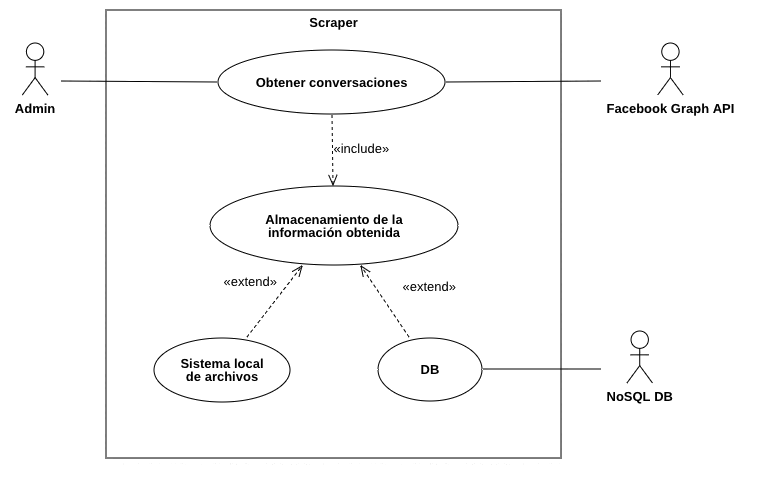
\includegraphics[height=10cm, width=16.5cm]{Latex/Classes/Imagenes/Scraper_cu.png}
             \caption{Diagrama de casos de uso para el modulo de extracción denominado \texit{Scraper}.}
             \label{fig:cu-scraper}
        \end{figure}
        La figura \ref{fig:cu-nlp-tp} describe una de las funcionalidades del modulo de procesamiento de lenguaje natural, en esta parte del proceso se trata de establecer una conexión con la base de datos no relacional donde los datos crudos obtenidos por \textit{Scraper} han sido almacenados, una vez que se han recuperados estos datos se realizada un paso denominado estandarización de texto, en el cual con ayuda de diccionarios de lemas y \textit{stopwords} se limpian los documentos dejando únicamente aquellas palabras relevantes, este proceso tiene muchas fases y cada una de estas son almacenadas en una base de datos relacional (véase la figura 4.7).
        \begin{figure}[H]
             \centering
             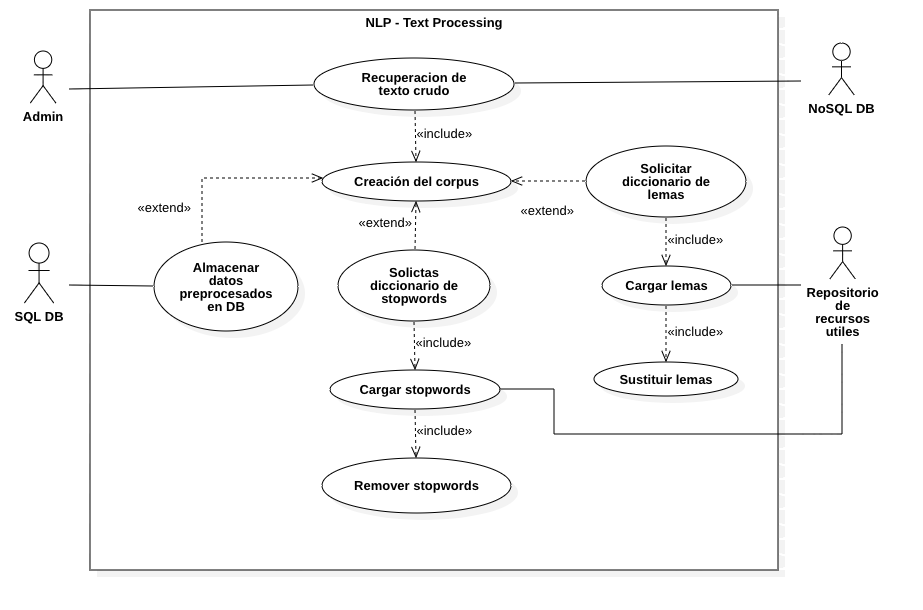
\includegraphics[height=14cm, width=16.5cm]{Latex/Classes/Imagenes/NLP_Text_Processing.png}
             \caption{Diagrama de casos de uso para el modulo de pre-procesamiento de texto.}
             \label{fig:cu-nlp-tp}
        \end{figure}
        La figura \ref{fig:cu-nlp-ta} describe otra de las funcionalidades del modulo de procesamiento de lenguaje natural, en el cual se obtienen los datos preprocesados de la base de datos relacional para aplicar el algoritmo \textbt{LDA} y poder extraer los temas frecuentes tratados dentro del texto.
        \begin{figure}[H]
             \centering
             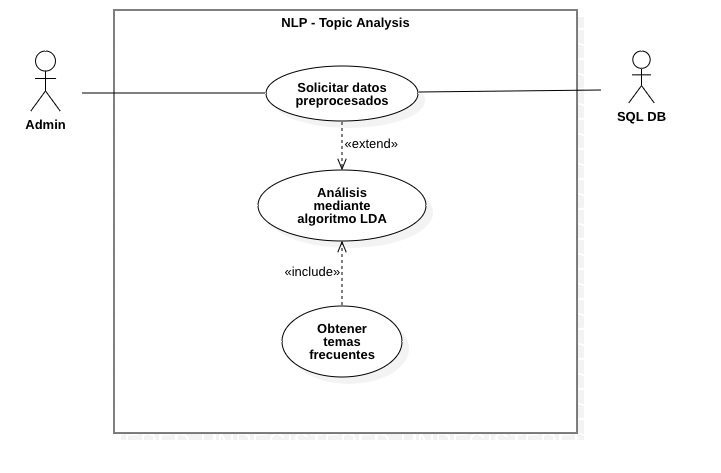
\includegraphics[height=8cm, width=16.5cm]{Latex/Classes/Imagenes/NLP_Topic_Analysis.png}
             \caption{Diagrama de casos de uso para el modulo de \textit{topic analysis}.}
             \label{fig:cu-nlp-ta}
        \end{figure}
        La figura \ref{fig:cu-nlp-g} describe la funcionalidad de graficación del modulo de procesamiento de lenguaje natural, el cual toma los datos que el algoritmo \textbf{LDA} arroja para graficarlos y que el usuario administrador pueda realizar un análisis visual de estos datos.
        \begin{figure}[H]
             \centering
             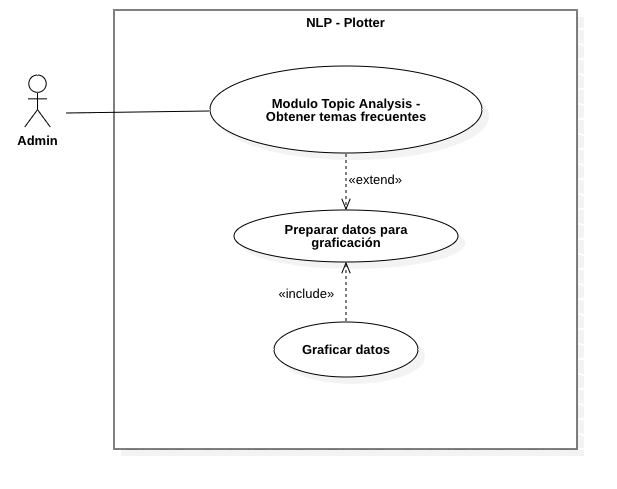
\includegraphics[height=8cm, width=16.5cm]{Latex/Classes/Imagenes/NLP_Plotter.png}
             \caption{Diagrama de casos de uso para el modulo de graficación.}
             \label{fig:cu-nlp-g}
        \end{figure}

    \subsection{Diagramas de procesos}
    Estos diagramas sirven para representar de manera gráfica un algoritmo o proceso. La figura \ref{fig:dp-scraper} muestra con mas detalle la funcionalidad del modulo \textit{Scraper} o de extracción. En primer lugar, este modulo espera recibir una serie de variables de entorno y banderas de entrada por parte del usuario, si la bandera de ``ayuda'' es percibida se muestra un mensaje de como usar el programa y se termina la ejecución, si no, entonces comienza el mapeo del resto de banderas, cabe destacar que estas banderas tienen un valor por defecto si el usuario no ingresa alguna. Una vez hecho esto entonces se busca por la bandera ``base de datos'', la cual si se encuentra en ``verdadero'' intentara establecer una conexión con la base de datos para almacenar ahí los mensajes, en dado caso de que la conexión no sea exitosa esta bandera automáticamente se cambia a ``flaso'' para prevenir futuros fallos y este registro se guarda en el sistema de \textit{logs}. Posteriormente se intenta establecer una conexión con \textit{Graph API}, si el \textit{token} es invalido se muestra un mensaje de error personalizado, se termina la ejecución y este error es almacenado en el sistema de \textit{logs}, en caso de una conexión exitosa comienza la descarga de mensajes, por cada mensaje se pregunta por la bandera de \textit{base de datos} para que, en caso de estar en ``verdadero'', el mensaje sea almacenado en la base de datos no relacional, de lo contrario el mensaje será almacenado en el sistema local de archivos. Una vez terminada la descarga de mensajes se termina la ejecución de este módulo. \break \break
    La figura \ref{fig:dp-nlp} muestra el flujo del módulo de procesamiento de lenguaje natural. En primer lugar, este modulo espera recibir una serie de variables de entorno y banderas de entrada por parte del usuario, si la bandera de ``ayuda'' percibida se muestra un mensaje de como usar el programa y se termina la ejecución, si no, entonces comienza el mapeo del resto de banderas, cabe destacar que estas banderas tienen un valor por defecto si el usuario no ingresa alguna. Posteriormente se intenta conectar con la base de datos relacional, en caso de una conexión fallida se muestra un mensaje de error personalizado, el registro se guarda en el sistema de \textit{logs} y se termina la ejecución, de lo contrario, busca que la bandera de \textit{pre-procesamiento} se encuentre en ``verdadero'', de ser así se intenta establecer una conexión con la base de datos no relacional, dándose el caso de una conexión fallida se muestra un mensaje de error personalizado, el registro se guarda en el sistema de \textit{logs} y se termina la ejecución, de lo contrario, se descargan los mensajes en su formato crudo para que por medio de diccionarios de lemas y \textit{stopwords} estos datos sean normalizados, cada uno de estos mensajes será guardado en la base de datos relacional. Luego, si la bandera de \textit{análisis LDA} se encuentra en ``verdadero'' y dada la columna de la base de datos relacional (véase la figura \ref{fig:diagrama-entidad-relacion}) especificada en las opciones de entrada, se procederá a descargar estos datos para realizar el análisis de tópicos, de lo contrario se finalizara la ejecución. Una vez realizado el análisis con el algoritmo \textbf{LDA} se pregunta si la bandera de \textif{graficación} esta en ``verdadero'', de ser así, entonces cada tópico propuesto por el algoritmo \textbf{LDA} sera graficado para realizar un análisis visual, en caso contrario los tópicos descubiertos serán almacenados en un archivo local para su futuro análisis, con este paso se terminal la ejecución del modulo de PLN.
        \begin{figure}[H]
             \centering
             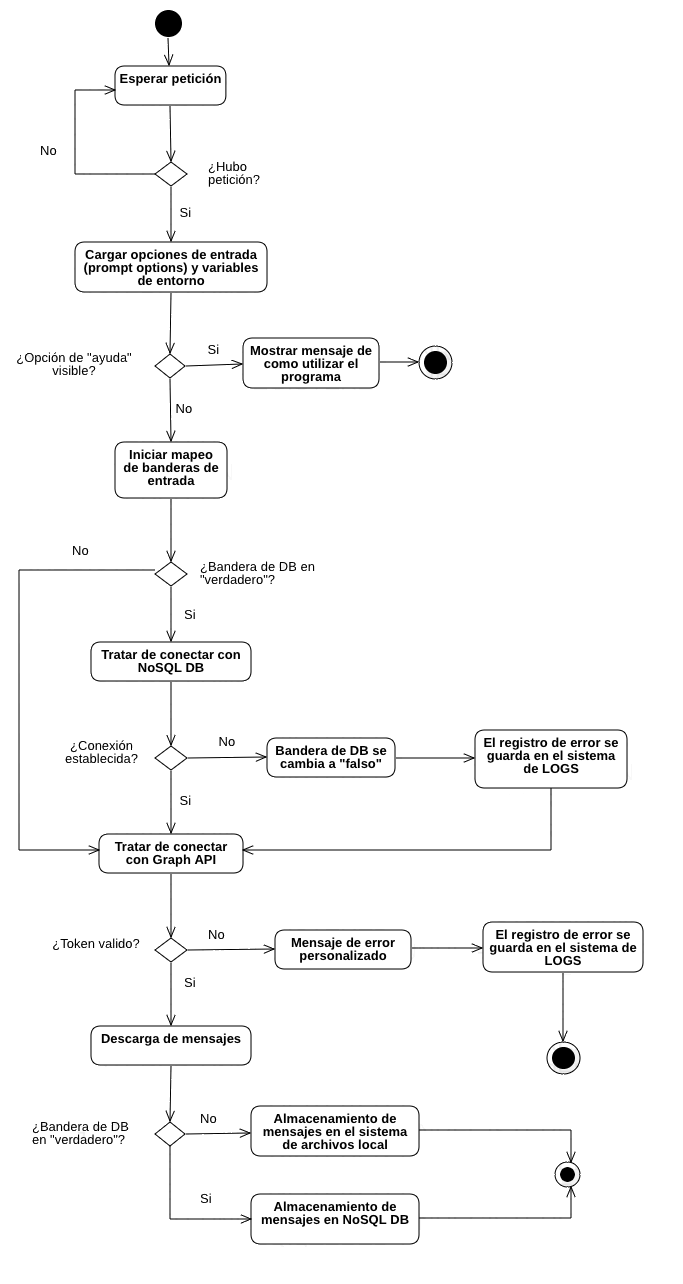
\includegraphics[height=18cm, width=16.5cm]{Latex/Classes/Imagenes/Scraper.png}
             \caption{Diagrama de procesos del módulo de extracción.}
             \label{fig:dp-scraper}
        \end{figure}
        \begin{figure}[H]
             \centering
             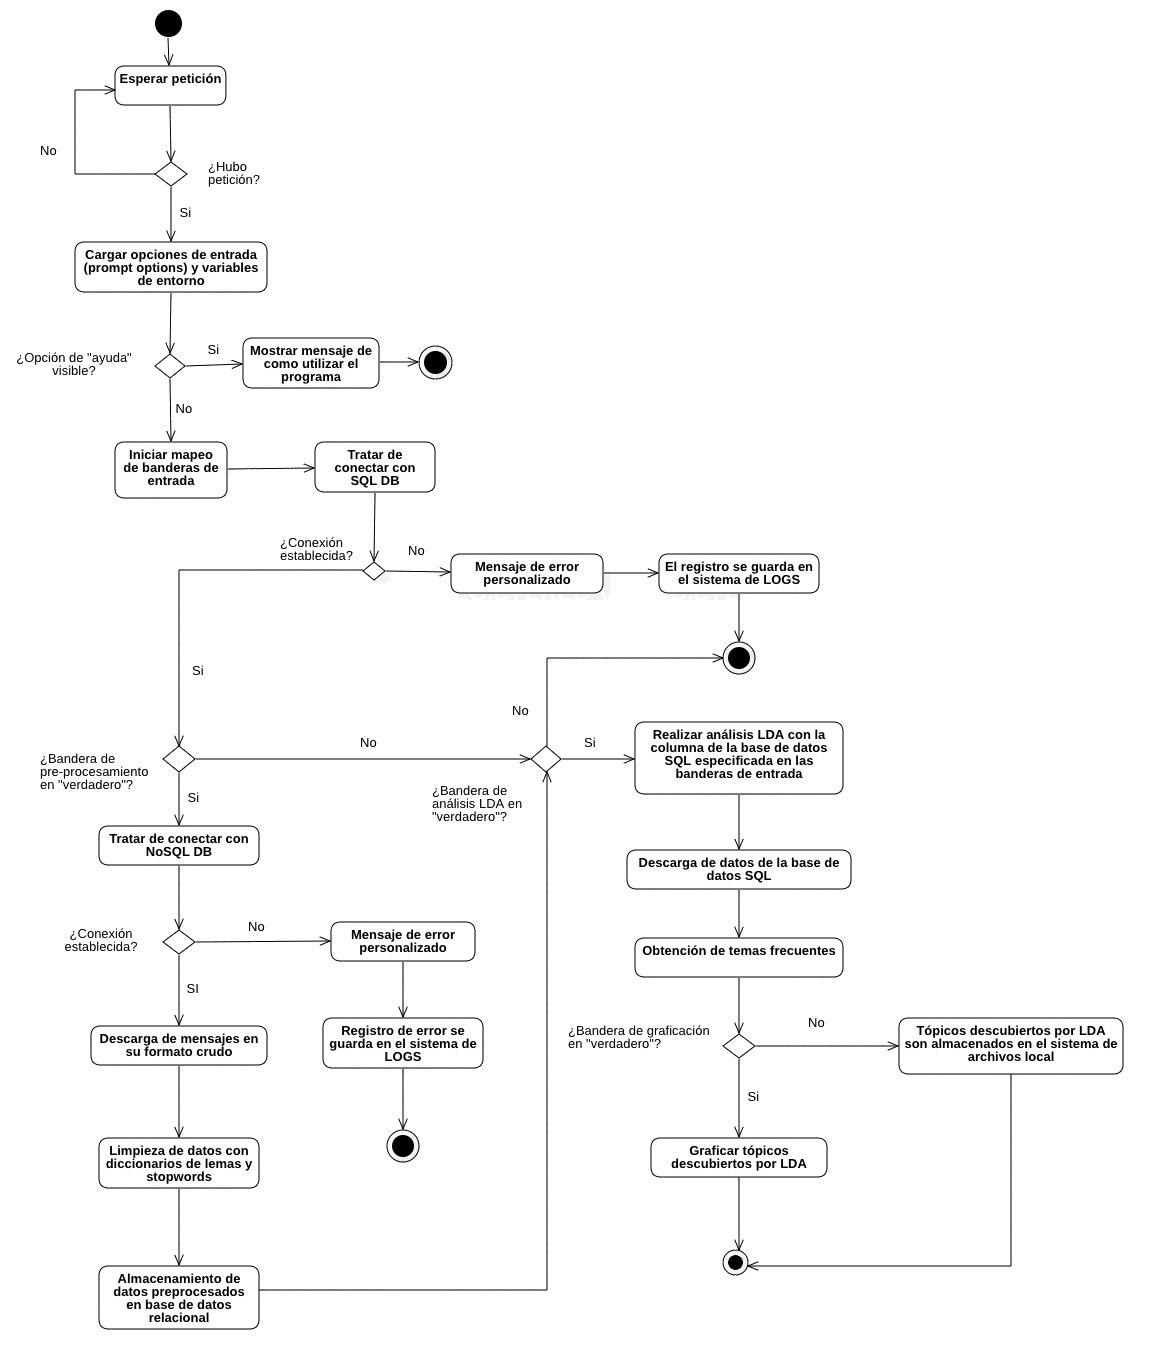
\includegraphics[height=20cm, width=16.5cm]{Latex/Classes/Imagenes/NLP.png}
             \caption{Diagrama de procesos del módulo de procesamiento de lenguaje natural.}
             \label{fig:dp-nlp}
        \end{figure}

    \subsection{Diagramas Entidad - Relación}
    El siguiente diagrama entidad-relación describe la base de datos relacional que será utilizada por el modulo de procesamiento de lenguaje natural, dicha base de datos cuenta únicamente con 2 tablas; \textit{Conversation}, que gurda una referencia de la conversación a la cual cada mensaje pertenece y \textit{Message} que almacena el mensaje en su formato crudo así como en distintos niveles de normalización.
    \begin{figure}[H]
         \centering
         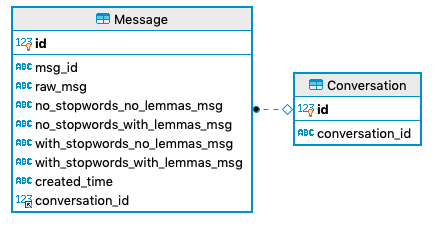
\includegraphics[width=.7\linewidth]{Latex/Classes/Imagenes/ER.png}
         \caption{Diagrama entidad-relación de la base de datos relacional.}
         \label{fig:diagrama-entidad-relacion}
    \end{figure}
    \newpage
        
    \subsection{Diagramas de clases}
        Los diagramas de clases mostrados en las figuras \ref{fig:dc-scraper} y \ref{fig:dc-nlp}, nos ayudan a entender de manera visual las clases que los módulos de \textit{extracción (scraper)} y \textit{procesamiento de lenguaje natural} utilizan, sus atributos, operaciones y las relaciones entre los objetos.
        \begin{figure}[H]
             \centering
             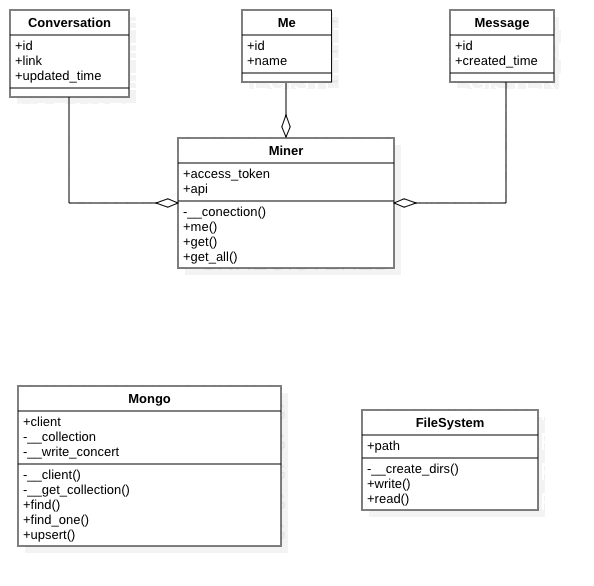
\includegraphics[height=9cm, width=16.5cm]{Latex/Classes/Imagenes/Scraper_Classes.png}
             \caption{Diagrama de clases del módulo \textit{Scraper} o de extracción.}
             \label{fig:dc-scraper}
        \end{figure}

        \begin{figure}[H]
             \centering
             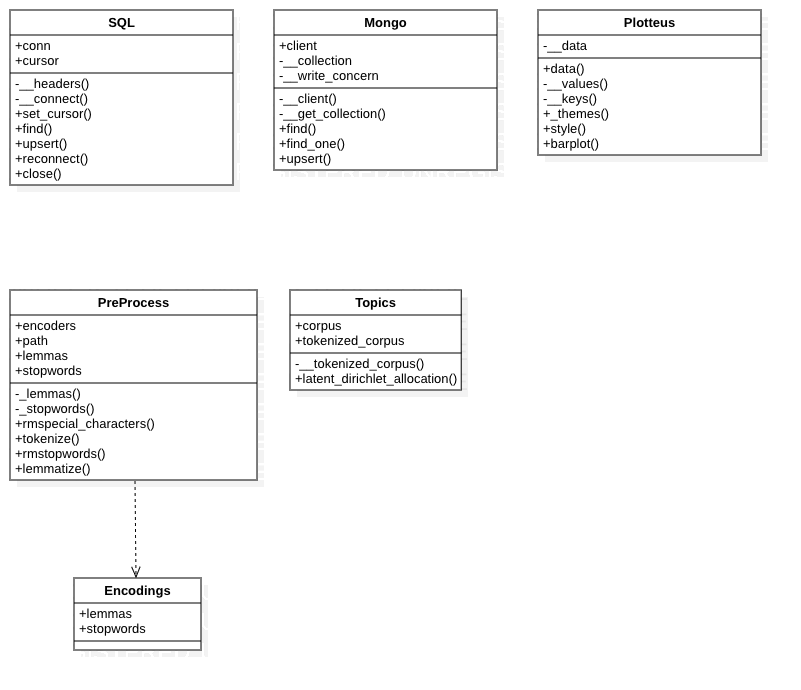
\includegraphics[height=9cm, width=16.5cm]{Latex/Classes/Imagenes/NLP_Classes.png}
             \caption{Diagrama de clases del módulo de procesamiento de lenguaje natural.}
             \label{fig:dc-nlp}
        \end{figure}
    \subsection{Diagramas de secuencia}
        El diagrama de secuencia de la figura \ref{fig:diagrama_secuencia} se muestra el proceso por el cual viaja una petición desde Facebook \textit{Graph API} hasta la infraestructura y como es tratado el dato:
        \begin{enumerate}
            \item La petición entra a una frontera \textit{AWS ACL} en el cual revisara que el no usuario se encuentre dentro de una black list
            \begin{enumerate}
                \item si esta: no permitirá el paso de trafico proveniente de ese usuario
                \item si no esta: redireccionará el trafico a \textit{API gateway}
                \begin{enumerate}

                    \item Llega a la frontera \textit{API gateway} el cual encolara la función control \textit{AWS Lambda} "StateMachine" dentro de la entidad \textit{AWS SQS}
                    \item La entidad \textit{AWS SQS} desencolara las anteriores peticiones de funciones control \textit{AWS Lambda} una por una de manera cronológica, "StateMachine" será desplegado al llegar al principio del encolador.
                    \item La función control \textit{AWS Lambda} "StateMachine" encolara dentro de una entidad \textit{AWS SQS} la función correspondiente al estado de la pregunta.
                    \begin{enumerate}
                        \item si el usuario es nuevo o nueva pregunta: la función a encolar será "Welcome"
                        \begin{enumerate}
                            \item La entidad \textit{AWS SQS} siguiendo el mismo principio del punto 3 invocará la funcion control \textit{AWS Lambda} "Welcome"
                            \item si el mensaje contenía una pregunta, se analizará y guardará el contexto dentro de la entidad \textit{AWS Elasticache}
                            \item La entidad \textit{AWS Elasticache} devolverá el estado de la petición a la funcion control \textit{AWS Lambda} "Welcome" tras haber guardado el contexto
                            \item La funcion control \textit{AWS Lambda} "Welcome" enviará la respuesta a la frontera \textit{API gateway}
                        \end{enumerate}
                        \item si es sobre preguntas pasadas: la función a encolar será "FAQs"
                        \begin{enumerate}
                            \item La entidad \textit{AWS SQS} siguiendo el mismo principio del punto 3 invocará la funcion control \textit{AWS Lambda} "FAQs"
                            \item La funcion control \textit{AWS Lambda} "FAQs" solicitará a la entidad \textit{AWS Elasticache} el contexto
                            \item La entidad \textit{AWS Elasticache} devolverá el contexto a la función control \textit{AWS Lambda} "FAQs"
                            \item La funcion control \textit{AWS Lambda} "FAQs" tras analizar la pregunta guardara el contexto dentro de la entidad \textit{AWS Elasticache}
                            \item si el mensaje contenía una pregunta, se analizará y guardará el contexto dentro de la entidad \textit{AWS Elasticache}
                            \item La entidad \textit{AWS Elasticache} devolverá el estado de la petición a la funcion control \textit{AWS Lambda} "FAQs" tras haber guardado el contexto
                            \item La funcion control \textit{AWS Lambda} "FAQs" enviará la respuesta a la frontera \textit{API gateway}
                        \end{enumerate}
                    \end{enumerate}
                    \item La frontera \textit{API gateway} actualizara las ACL de la frontera \textit{AWS ACL}
                    \item La frontera \textit{API ACL} se comunicará con Facebook \textit{Graph API} y retornara el resultado del análisis.
                    \item El paso 1.a.1 se repite hasta que la función control \textit{AWS Lambda} "StateMachine" pasa al estado "Fairwell"
                    \item La petición entra a una frontera \textit{AWS ACL} siguiendo la logica del paso 1
                    \item Llega a la frontera \textit{API gateway} el cual encolara la función control \textit{AWS Lambda} "StateMachine" dentro de la entidad \textit{AWS SQS}
                    \item La entidad \textit{AWS SQS} siguiendo el mismo principio del punto 3 invocará la funcion control \textit{AWS Lambda} "StateMachine"
                    \item La función control \textit{AWS Lambda} "StateMachine" encolara dentro de una entidad \textit{AWS SQS} la función "Fairwell"
                    \item Llega a la frontera \textit{API gateway} el cual encolara la función control \textit{AWS Lambda} "Fairwell" dentro de la entidad \textit{AWS SQS}
                     \item La funcion control \textit{AWS Lambda} "Fairwell" enviará la respuesta a la frontera \textit{API gateway}
                     \item La frontera \textit{API gateway} actualizara las ACL de la frontera \textit{AWS ACL}
                    \item La frontera \textit{API ACL} se comunicará con Facebook \textit{Graph API} y retornara la respuesta
                \end{enumerate}
            \end{enumerate}


            
            \item La entidad \textit{AWS SQS} desencolara los mensajes de forma ordenada lanzando otra función control \textit{AWS Lambda} para cada una de estas.
            \item La función control \textit{AWS Lambda} analizara la petición y buscará en la entidad \textit{AWS Elacticache} un contexto de preguntas pasadas.
            \item La entidad \textit{AWS Elasticache} buscara si existe un contexto previo, si existe entonces retornará este, en caso contrario solo mandará una notificación.
            \item La función control \textit{AWS Lambda} analizara el mensaje obtenido con base en el resultado de la entidad \textit{AWS Elacticache}  y devolverá el resultado a la frontera \textit{API gateway}.
            \item La frontera \textit{API gateway} se comunicará con Facebook \textit{Graph API} y retornara el resultado del análisis.
        \end{enumerate}
        
        \begin{figure}[H]
             \centering
             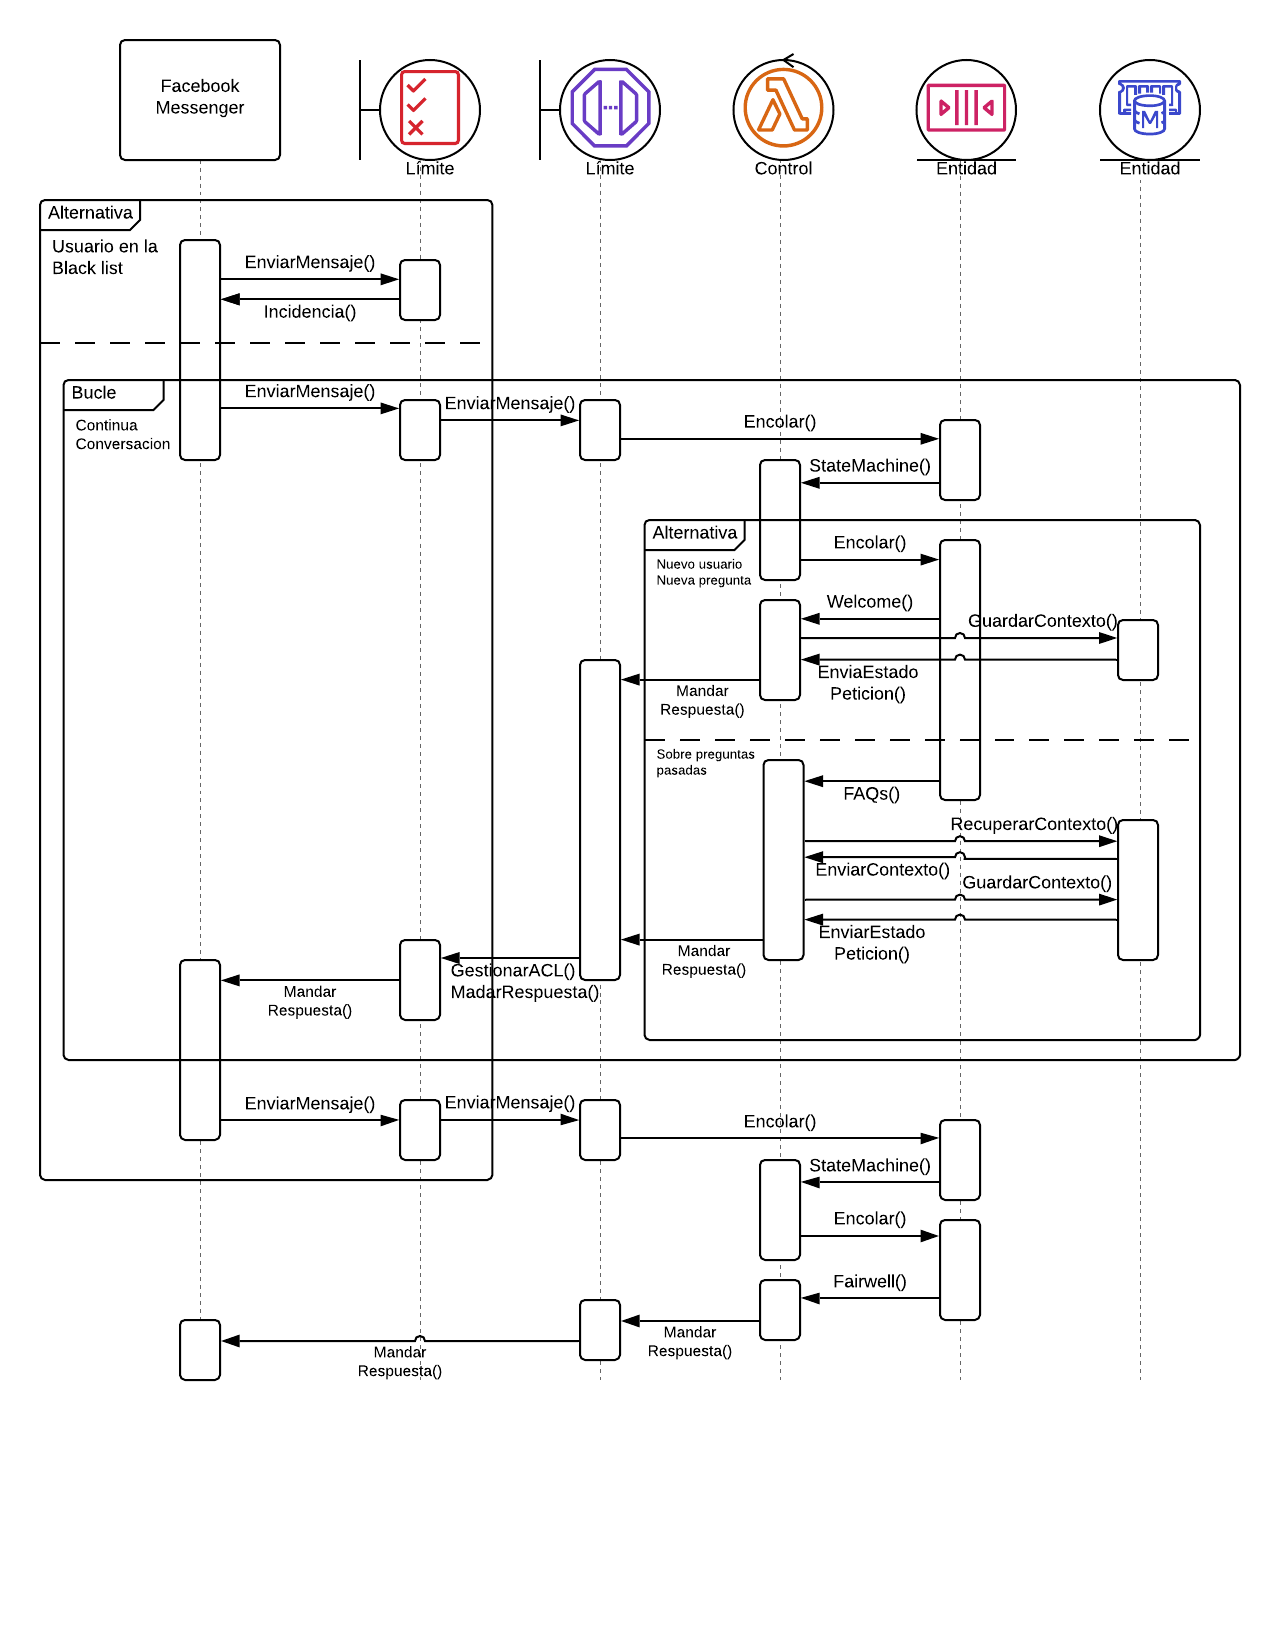
\includegraphics[height=14cm, width=16.5cm]{Latex/Classes/Imagenes/Diagrama_de_secuencia_del_sistema.png}
             \caption{Secuencia por la que viaja una pregunta dentro de las tecnologías de \textit{AWS}.}
             \label{fig:diagrama_secuencia}

        \end{figure}
    
    \subsection{Diagramas de infraestructura}
    
        El diagrama de infraestructura de la figura ~\ref{fig:infraestructura} se muestra la infraestructura sobre la cual se ejecutará el prototipo de agente conversacional, la implementación de este sera sobre el proveedor de computo en la nube \textit{AWS}.
        
        \textit{AWS Route 53} proveerá de los certificados necesarios para poder comunicar la tecnología \textit{AWS API Gateway} con Facebook \textit{Graph API} por medio de un canal bidireccional con las funciones de \textit{AWS Lambda} para mandar y recibir peticiones. \textit{AWS Lambda} ejecutará bloques de código cuando sea invocado retornando un resultado, \textit{AWS SQS} proveerá un sistema de encolamiento de mensajes de las peticiones entrantes y se definirá la acción de invocar una función de \textit{AWS Lambda} a la hora de desencolar estos. \textit{AWS Elasticache} proveerá una memoria temporal definida por el administrador, en el que se almacenan objetos de alta transaccionalidad de tipo clave valor. En el ambiente de despliegue, si se realiza un cambio sobre el código de una función de \textit{AWS Lambda} está se actualizará y se desplegara de tal manera que las nuevas funciones de \textit{AWS Lambda} corran con estos cambios.
        \begin{figure}[H]
             \centering
             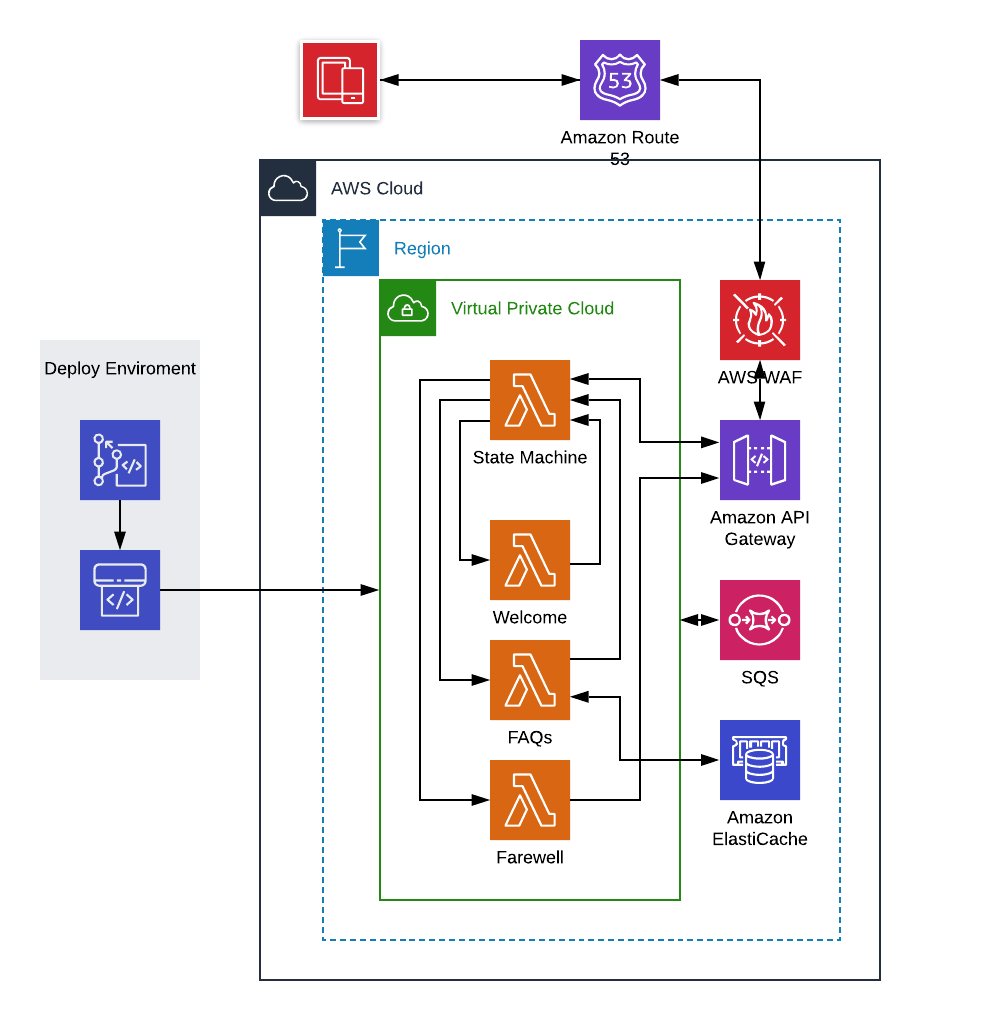
\includegraphics[height=12cm, width=16.5cm]{Latex/Classes/Imagenes/Diagrama_de_infraestructura.png}
             \caption{Infraestructura del agente conversacional}
             \label{fig:infraestructura}
        \end{figure}
        
        El diagrama de infraestructura de la figura  ~\ref{fig:infraestructuraExtraccionNLP} muestra dos módulos del prototipo de agente conversacional: Extracción y procesamiento de lenguaje natural.
        En el modulo de extracción se hace uso de un equipo de cómputo con salida a internet, se comunicará con \textit{Graph API} y obtendrá los datos pertinentes, sobre este equipo se ejecutará un contenedor de Docker con persistencia en el que correrá una base de datos NoSQL en una subnet privada con comunicación de tipo puente con el equipo de cómputo y se almacenarán los datos obtenidos.
        En el modulo de NLP, se hace uso de un equipo de cómputo en el que se ejecutarán dos contenedores con persistencia en una subnet privada con comunicación de tipo puente con el equipo de cómputo, los datos almacenados en la base de datos NoSQL pasaran por un submodulo de preprocesado y serán almacenados en la base de datos SQL. Con base a estos datos se ejecutará el submodulo de análisis de tópicos, al finalizar se comunicara internamente con el equipo y este ejecutará el submodulo de graficación.
        \begin{figure}[H]
             \centering
             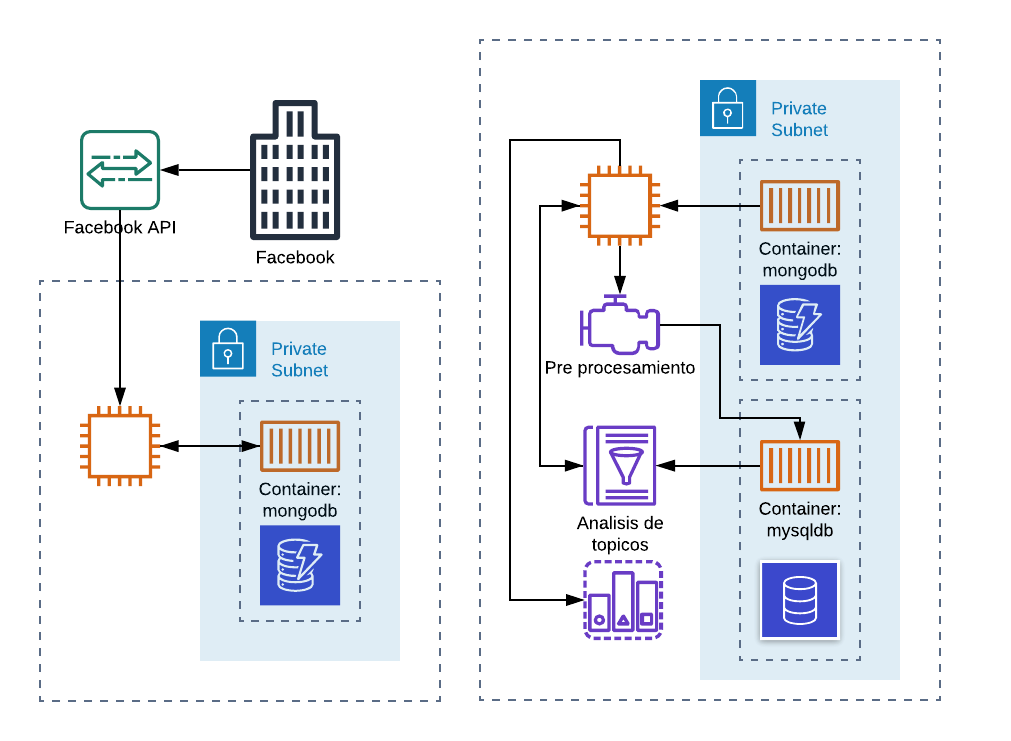
\includegraphics[height=12cm, width=16.5cm]{Latex/Classes/Imagenes/Diagramas_de_modulos.png}
             \caption{Infraestructura de los modulo de extracción y NLP respectivamente}
              \label{fig:infraestructuraExtraccionNLP}

        \end{figure}
    \subsection{Construcción del modelo}
    
        Es importante remarcar el hecho de que nuestro agente conversacional estará basado en un dominio de espacio cerrado enfocado a la resolución de preguntas frecuentes correspondientes al área de administración educativa, las respuestas obtenidas por este, estarán basadas en un modelo generativo.
        Se plantea el uso de mecanismos de atención el cual se encargará de dirigir la conversación hacia una pregunta especifica.
        
        La arquitectura interna del modelo esta basada en \it{Seg2Seg} el cual cuenta con tres capas de redes neuronales recurrentes con diferentes conjuntos de parámetros, una capa se encargará de codificar la secuencia de la fuente y la otra en decodificar la secuencia codificada por la anterior red neuronal 
        
        \begin{description}
        \item [Codificador:] Se encarga de obtener los datos de la pregunta y se entrenará con ellos, pasando la información a cada una se sus neuronas por medio de una cinta de memoria, al llegar al final, se mandará el estado junto con una cadena de inicio a la siguiente red neuronal, a partir de estos datos se generaran las respuestas.
        \end{description}
        \begin{figure}[H]
             \centering
             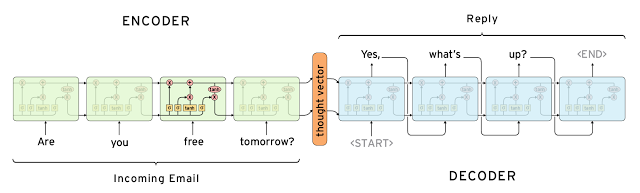
\includegraphics[height=7cm, width=16.5cm]{Latex/Classes/Imagenes/seg2seg.png}
             \caption{Arquitectura \it{Seg2Seg}}
              \label{fig:infraestructuraExtraccionNLP}
        \end{figure}
        
        Las redes neuronales dentro de estas dos capas son del tipo \it{LSTM} los cuales son una variante de las \it{RRN}, cuentan con una célula de memoria el cual esta compuesta por 3 principales compuertas:
        
        
        \begin{description}
            \item [Forget gate:] se encarga de analizar la entrada junto al estado de la \it{LSTM}, y pasar estos por medio de una fusión de activación de tipo \it{sigmoidal}, se eliminaran los datos que no serán usados en adelante.
            \item [Output gate:] después de aplicar las transformaciones de la cinta con la salida de la \it{Forget gate} y transformando esta con el resultado de \it{Update gate}, transformaremos el resultado con una función \it{Tanh} a la cinta de memoria y la pasaremos por una compuerta \bf{XOR} con la entrada junto al estado de la \bf{LSTM}, ya pasados por la fusión de activación de tipo \it{sigmoidal}, generaremos así la salida del nuevo estado.
        \end{description}
        
          \begin{figure}[H]
             \centering
             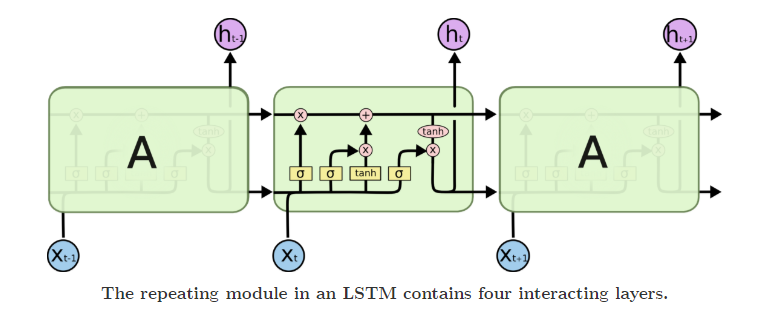
\includegraphics[height=7cm, width=16.5cm]{Latex/Classes/Imagenes/LSTM.png}
             \caption{Arquitectura de la LSTM}
              \label{fig:infraestructuraExtraccionNLP}
        \end{figure}
        
        La tercera capa es un mecanismo de atención, enfocado en generar respuestas recomendadas con base al contexto de los estados de cada neurona del codificador junto a la intención obtenida por el modulo de \it{LDA}. 
        \begin{figure}[H]
             \centering
             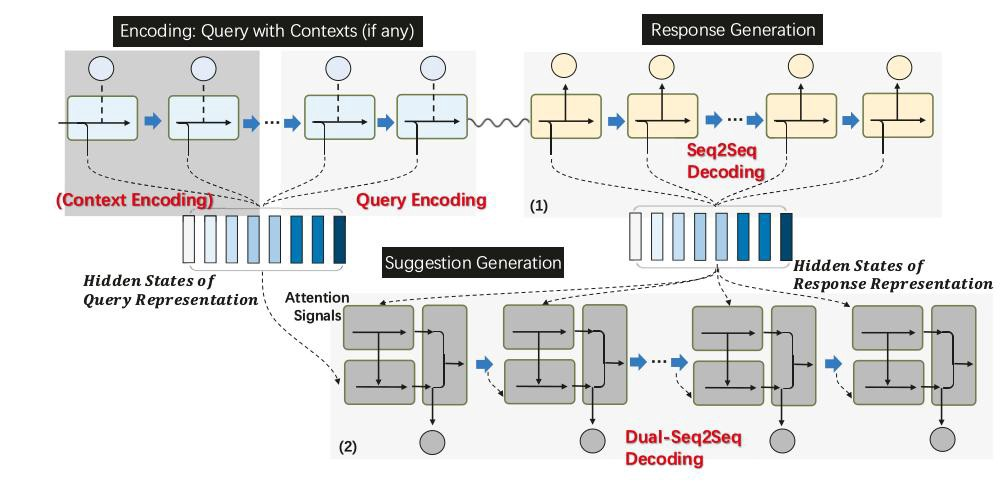
\includegraphics[height=12cm, width=16.5cm]{Latex/Classes/Imagenes/attention.jpeg}
             \caption{Arquitectura del mecanismo de atención}
              \label{fig:infraestructuraExtraccionNLP}
        \end{figure}
    \subsection{Resultados esperados}
        \begin{figure}[H]
             \centering
             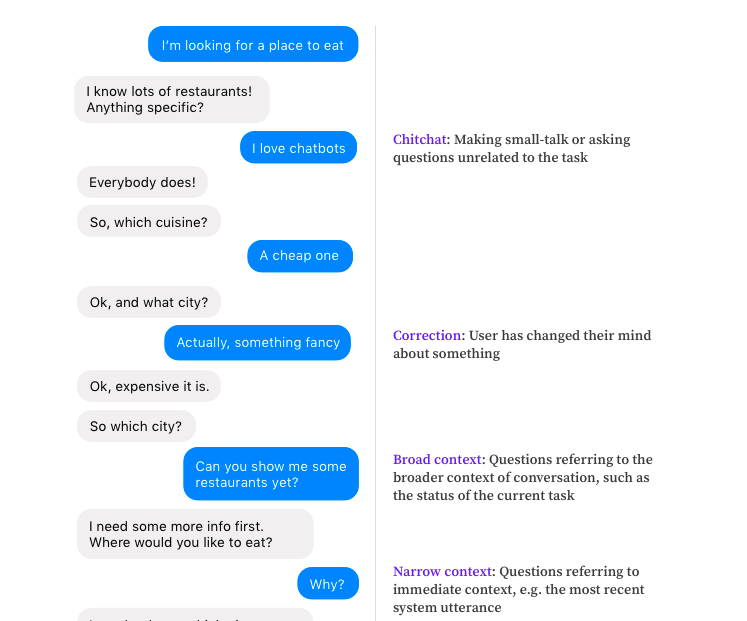
\includegraphics[height=12cm, width=16.5cm]{Latex/Classes/Imagenes/hola.png}
             \caption{Resultados esperados usando la técnica de \it{Seg2Seg} con mecanismos de atención}
              \label{fig:infraestructuraExtraccionNLP}
        \end{figure}
        
    Cabe destacar que este modelo estará delimitado por una cierta cantidad de preguntas a resolver, como ya se menciono, será un sistema cerrado enfocándose principalmente en 3 tipos de peticiones:
    
    \begin{itemize}
        \item Convocatorias de inscripción, tanto semestrales como Trabajos Terminales, protocolo de TT, electiva, optativa y postgrados.
        \item Información para la baja de unidades de aprendizaje así como baja temporal o definitiva.
        \item Información general para alumnos de nuevo ingreso sobre la Escuela Superior de Cómputo.
    \end{itemize}
\chapter{Resultados}
    Con el fin de demostrar la correcta funcionalidad de los módulos descritos en el capitulo 4, en el presente apartado se exponen los diversos resultados obtenidos a lo largo del desarrollo del prototipo. Por discreción, los datos sensibles fueron enmascarados.
    
    \section{Módulo de extracción (\textit{Scraper})}
    Este módulo basa su funcionalidad en la conectividad exitosa con \textit{Graph API} de Facebook para poder dar lugar a la descarga de conversaciones que serán empleadas por el agente conversacional después de haber sido normalizadas. Como se menciono en la sección 4, al descargar las conversaciones se busca que exista una base de datos no relacional disponible, de ser así entonces las conversaciones serán almacenadas en dicha base de datos (figura \ref{fig:almacenamiento-db-nosql}), en caso contrario en el sistema local de archivos (figura \ref{fig:almacenamiento-local-conversacion}, \ref{fig:almacenamiento-local-mensaje} y \ref{fig:almacenamiento-local-mensaje-editor}).
    
    \begin{figure}[H]
         \centering
         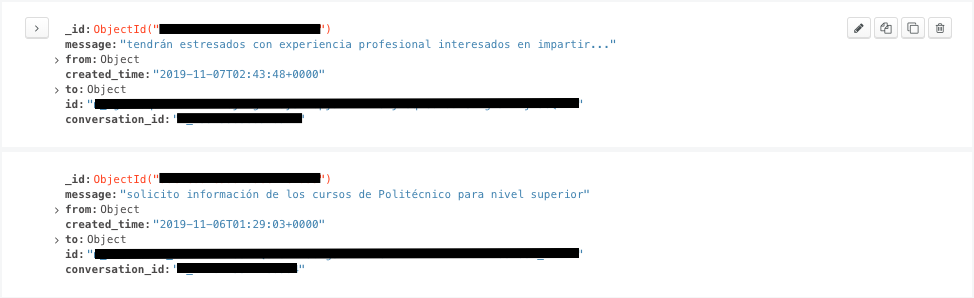
\includegraphics[height=7cm, width=16.5cm]{Latex/Classes/Imagenes/almacenamiento-db-nosql.png}
         \caption{Datos crudos obtenidos de \textit{Graph API} almacenados en base de datos \textit{NoSQL}.}
         \label{fig:almacenamiento-db-nosql}
    \end{figure}
    
    \begin{multicols}{2}
        \begin{figure}[H]
             \centering
             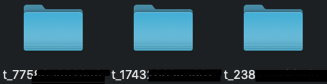
\includegraphics[height=2.5cm, width=6cm]{Latex/Classes/Imagenes/almacenamiento-local.png}
             \caption{Datos crudos obtenidos de \textit{Graph API} almacenados en el sistema local de archivos por conversación.}
             \label{fig:almacenamiento-local-conversacion}
        \end{figure}
        
        \begin{figure}[H]
             \centering
             
\includegraphics[height=2.5cm, width=6cm]{Latex/Classes/Imagenes/conversacion-local.png}
             \caption{Datos crudos obtenidos de \textit{Graph API} almacenados en el sistema local de archivos por mensaje.}
             \label{fig:almacenamiento-local-mensaje}
        \end{figure}
    \end{multicols}
    \begin{figure}[H]
         \centering
         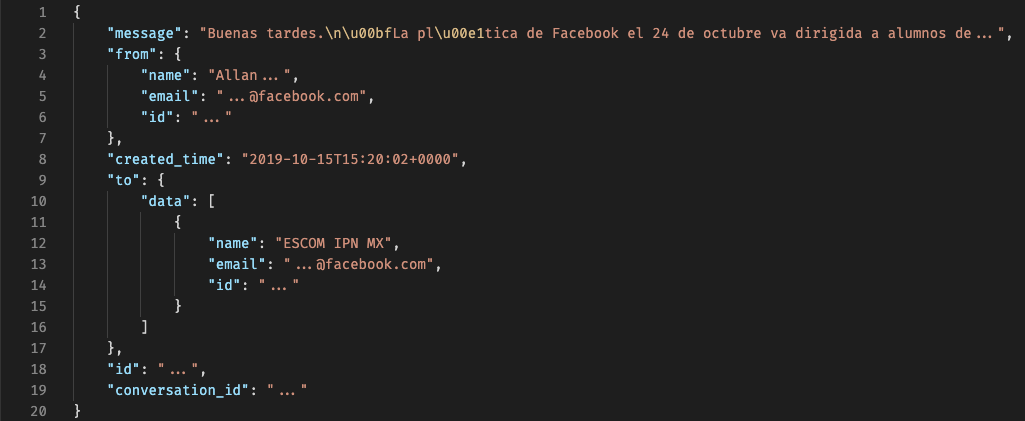
\includegraphics[height=6cm, width=16.5cm]{Latex/Classes/Imagenes/conversacion-local-vista.png}
         \caption{Datos crudos obtenidos de \textit{Graph API} almacenados en el sistema local de archivos visto desde un editor de texto.}
         \label{fig:almacenamiento-local-mensaje-editor}
    \end{figure}
    
    \section{Módulo de procesamiento de lenguaje natural}
    Una vez que se tiene una base de datos \textit{NoSQL} disponible y además, alimentada con los datos crudos gracias a \textit{Graph API}, el módulo de procesamiento de lenguaje natural hace disposición de estos datos para limpiarlos y almacenarlos en una base de datos relacional (véase la figura \ref{fig:diagrama-entidad-relacion}) en cada una de sus etapas de normalización como se puede ver en la figura \ref{fig:sql-message-table}, es decir:
    \begin{itemize}
        \item Mensaje crudo: Mensaje tal cual es extraído de \textit{Graph API}.
        \item Mensaje con stopwords y sin lemas: Mensaje sin cualquier carácter que no pertenezca al abecedario latino.
        \item Mensaje sin stopwords y sin lemas: Mensaje sin cualquier carácter que no pertenezca al abecedario latino y sin \textit{stopwords}.
        \item Mensaje sin stopwords y con lemas: Mensaje sin cualquier carácter que no pertenezca al abecedario latino, sin \textit{stopwords} y lematizado. 
        \item Mensaje con stopwords y con lemas: Mensaje sin cualquier carácter que no pertenezca al abecedario latino y lematizado. 
    \end{itemize}
    
    \begin{figure}[H]
         \centering
         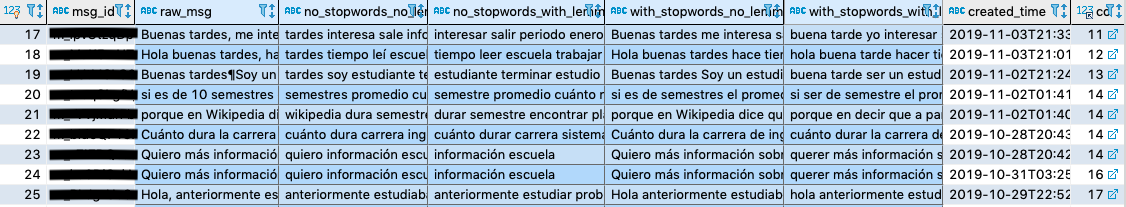
\includegraphics[height=4cm, width=16.5cm]{Latex/Classes/Imagenes/message-table.png}
         \caption{Datos en diferentes niveles de normalización almacenados en la base de datos relacional.}
         \label{fig:sql-message-table}
    \end{figure}

    \begin{figure}[H]
         \centering
         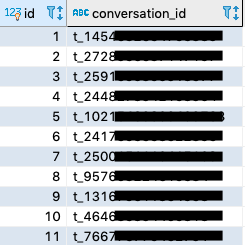
\includegraphics[height=6cm, width=8cm]{Latex/Classes/Imagenes/conversation-table.png}
         \caption{Tabla de conversaciones.}
         \label{fig:sql-conversation-table}
    \end{figure}
    
    Una vez realizada la normalización, se extraen los datos de cada una de las columnas descritas anteriormente para poder realizar un análisis de tópicos, a continuación se muestran los resultados. \newpage
    
    \begin{itemize}
        \item De los mensajes con \textit{stopwords} y sin lemas no se pudo obtener gran información puesto que las palabras que predominan son palabras vacías como artículos, pronombres, preposiciones, etc.
        \begin{figure}[H]
            \centering
            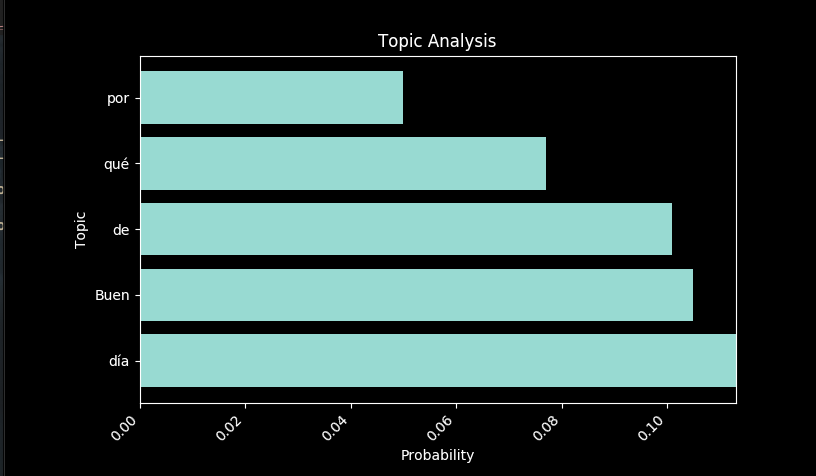
\includegraphics[height=8cm, width=16.5cm]{Latex/Classes/Imagenes/ws_nl-1.png}
            \caption{Resultado \textbf{LDA} con documentos con \textit{stopwords} y sin lemas (a).}
            \label{fig:ws_nl-1}
        \end{figure}
        \begin{figure}[H]
            \centering
            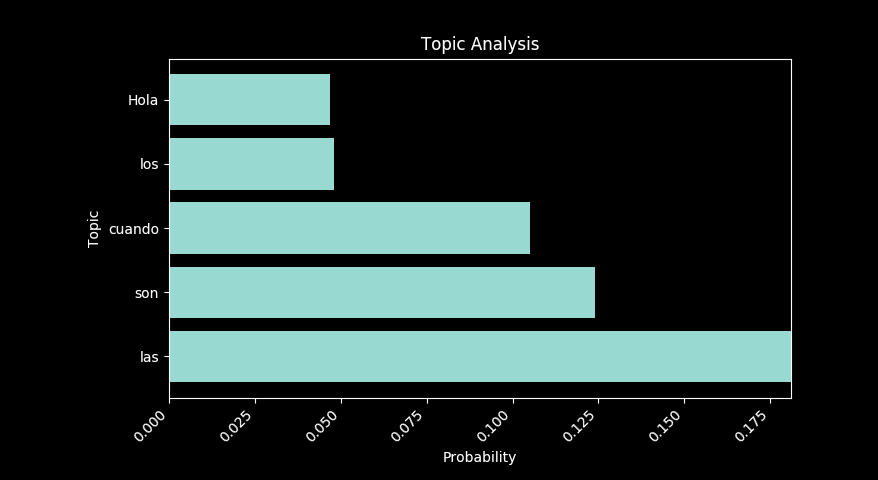
\includegraphics[height=8cm, width=16.5cm]{Latex/Classes/Imagenes/ws_nl-2.png}
            \caption{Resultado \textbf{LDA} con documentos con \textit{stopwords} y sin lemas (b).}
            \label{fig:ws_nl-2}
        \end{figure}
        \newpage
        
        \item De los mensajes con \textit{stopwords} y con lemas no se pudo obtener gran información puesto que las palabras que predominan siguen siendo palabras vacías como artículos, pronombres, preposiciones, etc., a pesar de que el texto se encuentre lematizado.
        \begin{figure}[H]
            \centering
            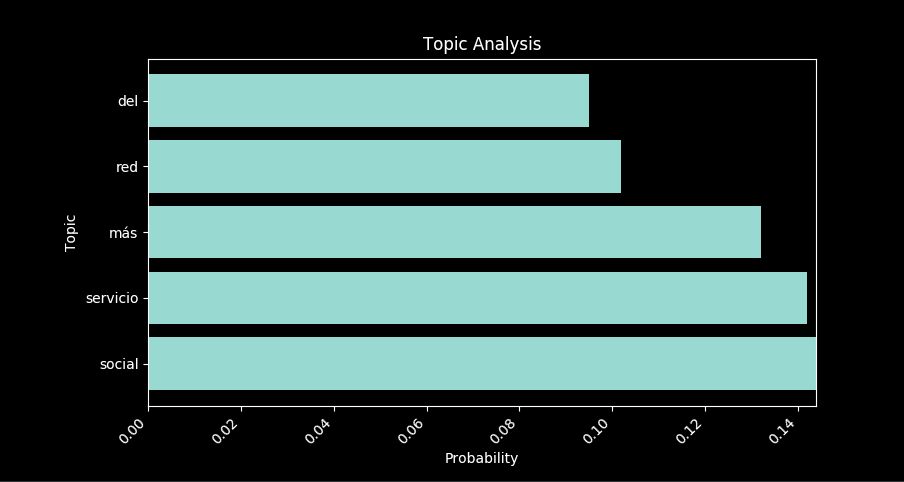
\includegraphics[height=8cm, width=16.5cm]{Latex/Classes/Imagenes/ws_wl-1.png}
            \caption{Resultado \textbf{LDA} con documentos con \textit{stopwords} y con lemas (a).}
            \label{fig:ws_wl-1}
        \end{figure}
        \begin{figure}[H]
            \centering
            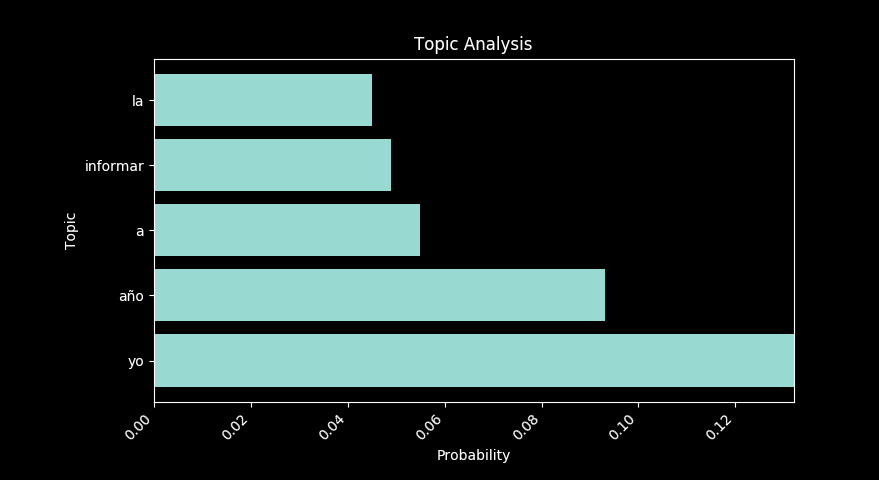
\includegraphics[height=8cm, width=16.5cm]{Latex/Classes/Imagenes/ws_wl-2.png}
            \caption{Resultado \textbf{LDA} con documentos con \textit{stopwords} y con lemas (b).}
            \label{fig:ws_wl-2}
        \end{figure}
        \newpage
        
        \item De los mensajes sin \textit{stopwords} y sin lemas los resultados obtenidos dieron lugar un avance significativo en los resultados, puesto que se pudieron encontrar temas relevantes de interés entre los estudiantes como: tramite de baja temporal, convocatorias de exámenes de admisión, inscripciones, información sobre el plantel e incluso ofertas laborales.
        \begin{figure}[H]
            \centering
            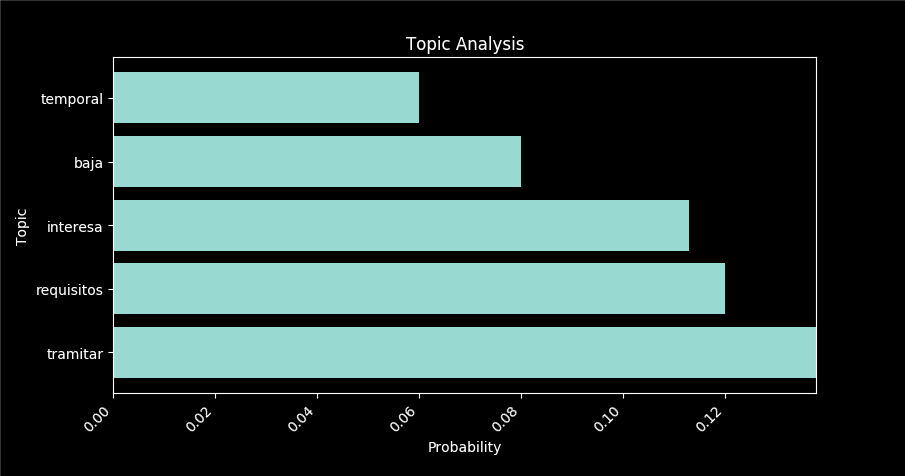
\includegraphics[height=8cm, width=16.5cm]{Latex/Classes/Imagenes/ns_nl-1.png}
            \caption{Resultado \textbf{LDA} con documentos sin \textit{stopwords} y sin lemas (a).}
            \label{fig:ns_nl-1}
        \end{figure}
        \begin{figure}[H]
            \centering
            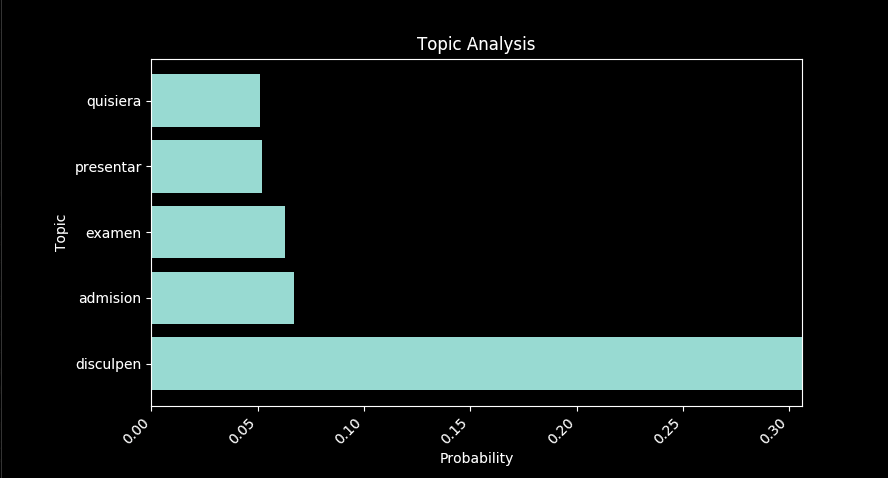
\includegraphics[height=8cm, width=16.5cm]{Latex/Classes/Imagenes/ns_nl-2.png}
            \caption{Resultado \textbf{LDA} con documentos sin \textit{stopwords} y sin lemas (b).}
            \label{fig:ns_nl-2}
        \end{figure}
        \begin{figure}[H]
            \centering
            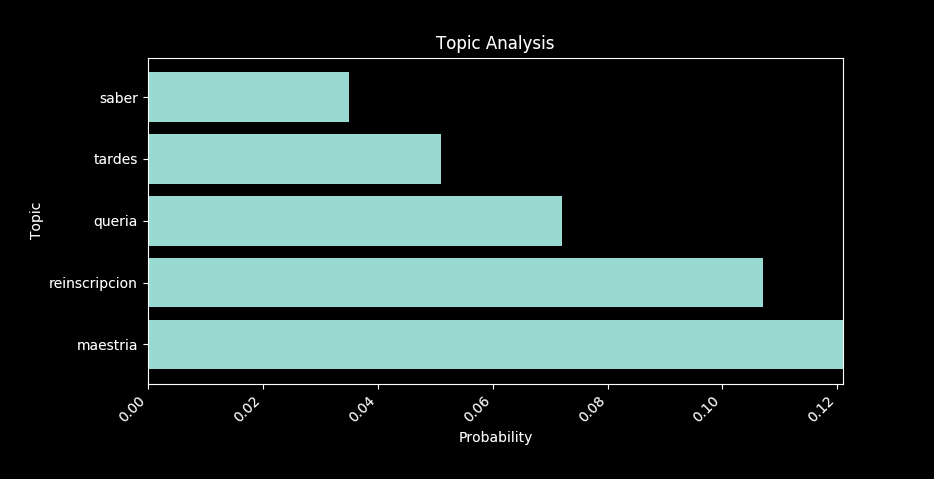
\includegraphics[height=8cm, width=16.5cm]{Latex/Classes/Imagenes/ns_nl-3.png}
            \caption{Resultado \textbf{LDA} con documentos sin \textit{stopwords} y sin lemas (c).}
            \label{fig:ns_nl-3}
        \end{figure}
        \begin{figure}[H]
            \centering
            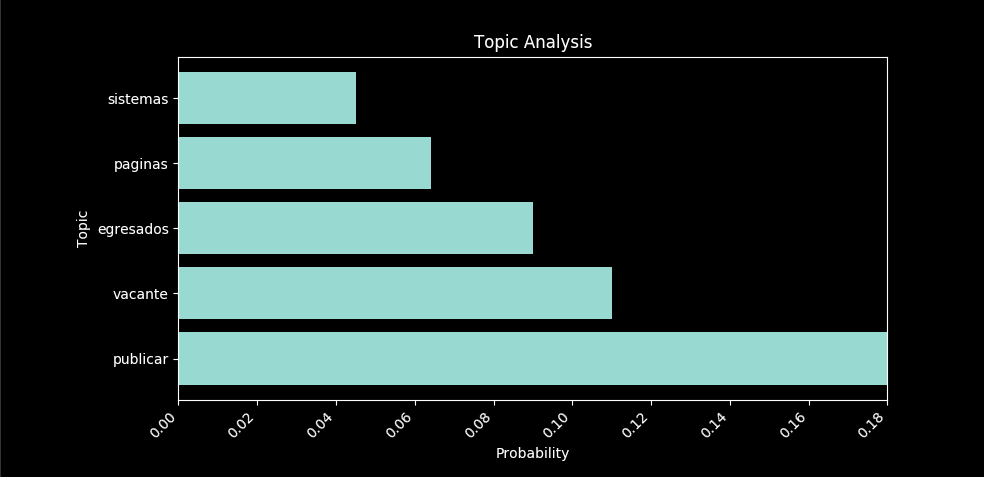
\includegraphics[height=8cm, width=16.5cm]{Latex/Classes/Imagenes/ns_nl-4.png}
            \caption{Resultado \textbf{LDA} con documentos sin \textit{stopwords} y sin lemas (d).}
            \label{fig:ns_nl-4}
        \end{figure}
        \begin{figure}[H]
            \centering
            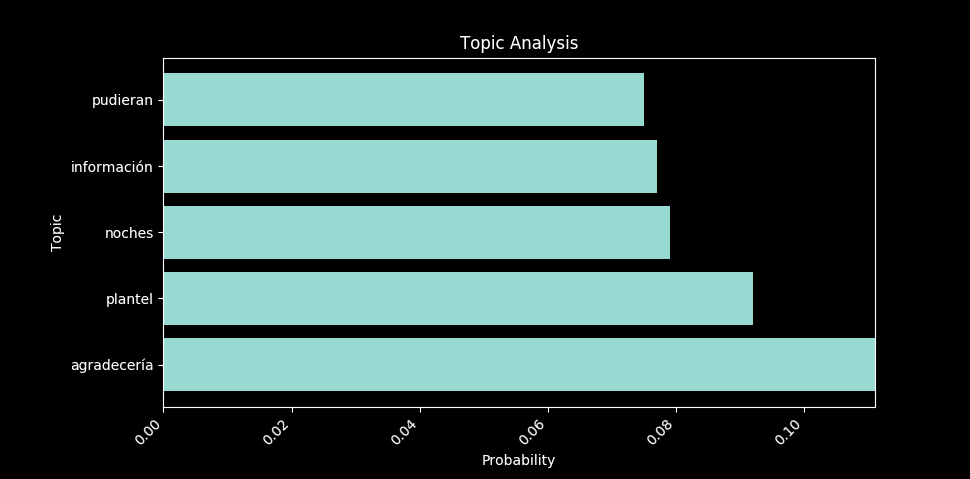
\includegraphics[height=8cm, width=16.5cm]{Latex/Classes/Imagenes/ns_nl-5.png}
            \caption{Resultado \textbf{LDA} con documentos sin \textit{stopwords} y sin lemas (e).}
            \label{fig:ns_nl-5}
        \end{figure}
        \begin{figure}[H]
            \centering
            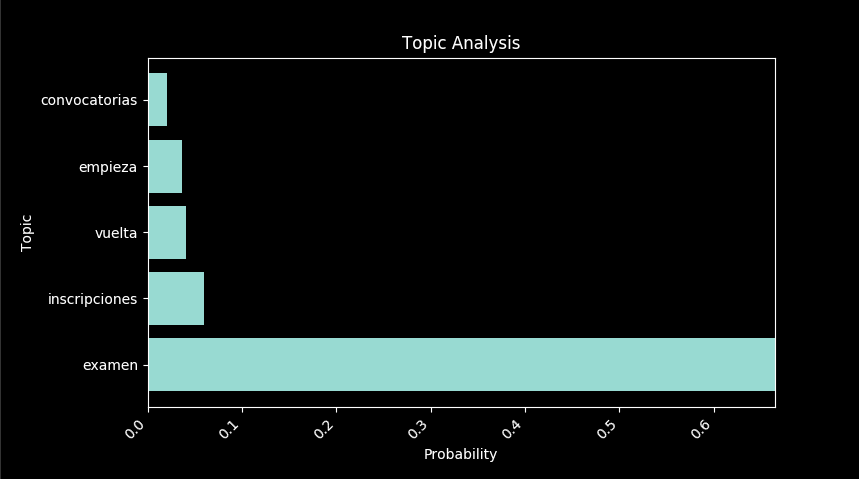
\includegraphics[height=8cm, width=16.5cm]{Latex/Classes/Imagenes/ns_nl-6.png}
            \caption{Resultado \textbf{LDA} con documentos sin \textit{stopwords} y sin lemas (f).}
            \label{fig:ns_nl-6}
        \end{figure}
        \newpage
        
        \item De los mensajes sin \textit{stopwords} y con lemas, probablemente dieron lugar a los resultados esperados ya que la mayoría de los estudiantes están interesados en los siguientes tópicos: exámenes de ingreso, cambio de carrera, convocatoria de titulación, convocatoria para inscripción a maestría, bajas temporales, taller de protocolo de trabajo terminal, servicio social, etc.
        \begin{figure}[H]
            \centering
            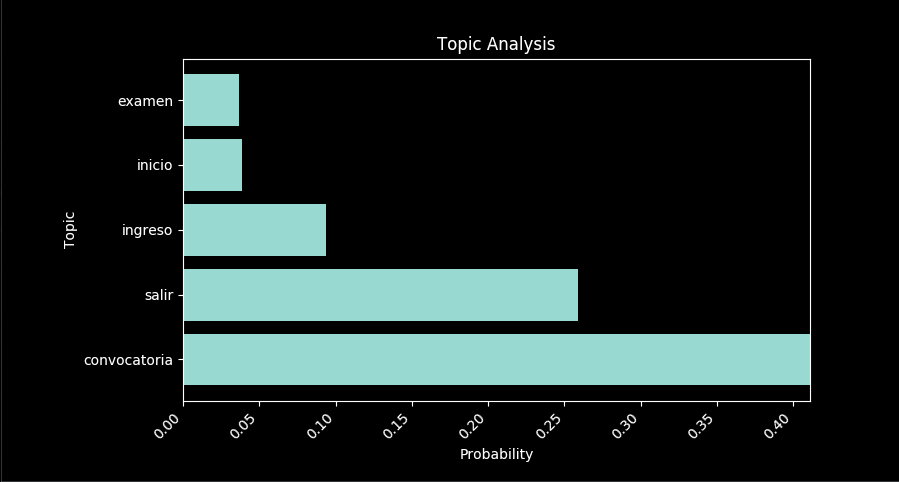
\includegraphics[height=8cm, width=16.5cm]{Latex/Classes/Imagenes/ns_wl-1.png}
            \caption{Resultado \textbf{LDA} con documentos sin \textit{stopwords} y con lemas (a).}
            \label{fig:ns_wl-1}
        \end{figure}
        \begin{figure}[H]
            \centering
            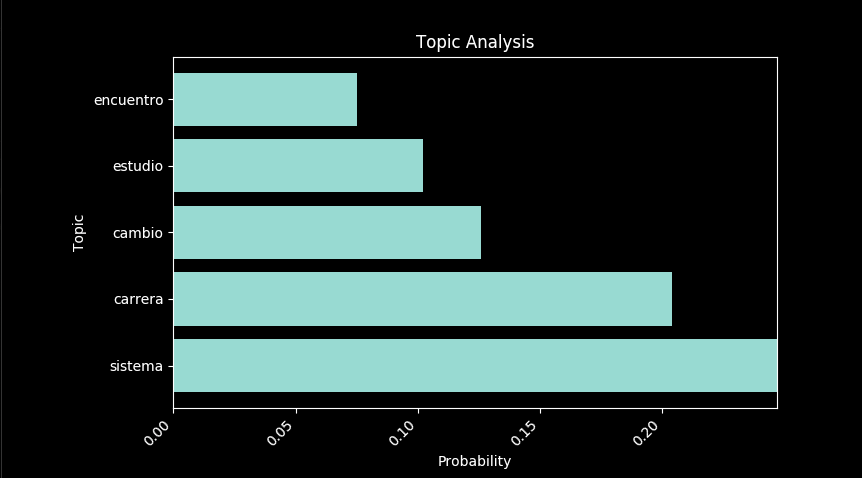
\includegraphics[height=8cm, width=16.5cm]{Latex/Classes/Imagenes/ns_wl-2.png}
            \caption{Resultado \textbf{LDA} con documentos sin \textit{stopwords} y con lemas (b).}
            \label{fig:ns_wl-2}
        \end{figure}
        \begin{figure}[H]
            \centering
            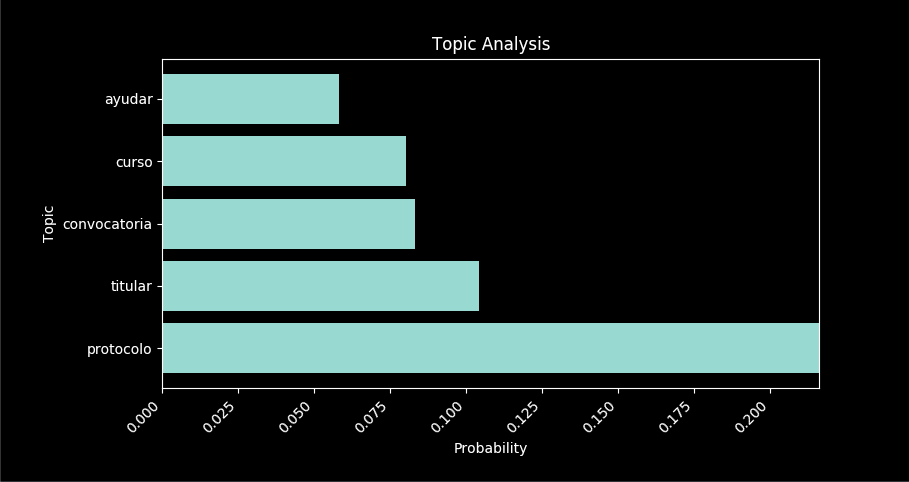
\includegraphics[height=8cm, width=16.5cm]{Latex/Classes/Imagenes/ns_wl-3.png}
            \caption{Resultado \textbf{LDA} con documentos sin \textit{stopwords} y con lemas (c).}
            \label{fig:ns_wl-3}
        \end{figure}
        \begin{figure}[H]
            \centering
            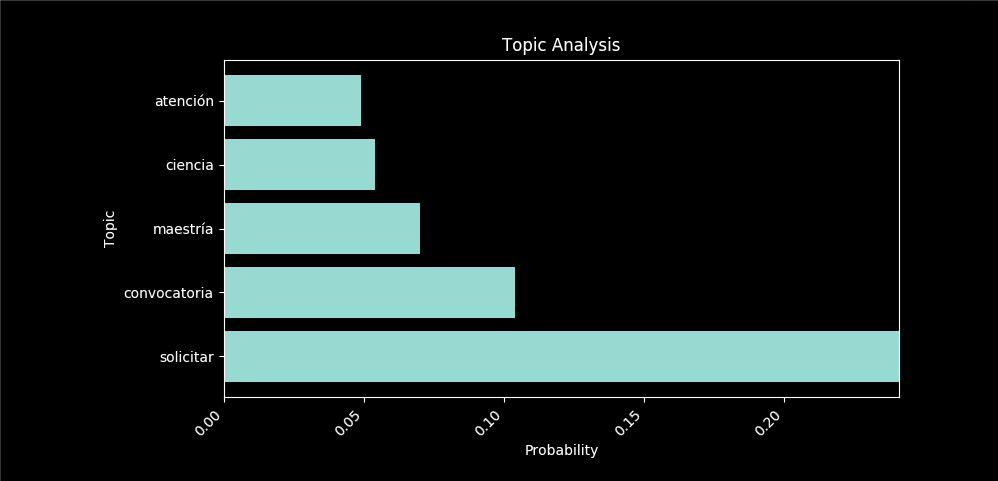
\includegraphics[height=8cm, width=16.5cm]{Latex/Classes/Imagenes/ns_wl-4.png}
            \caption{Resultado \textbf{LDA} con documentos sin \textit{stopwords} y con lemas (d).}
            \label{fig:ns_wl-4}
        \end{figure}
        \begin{figure}[H]
            \centering
            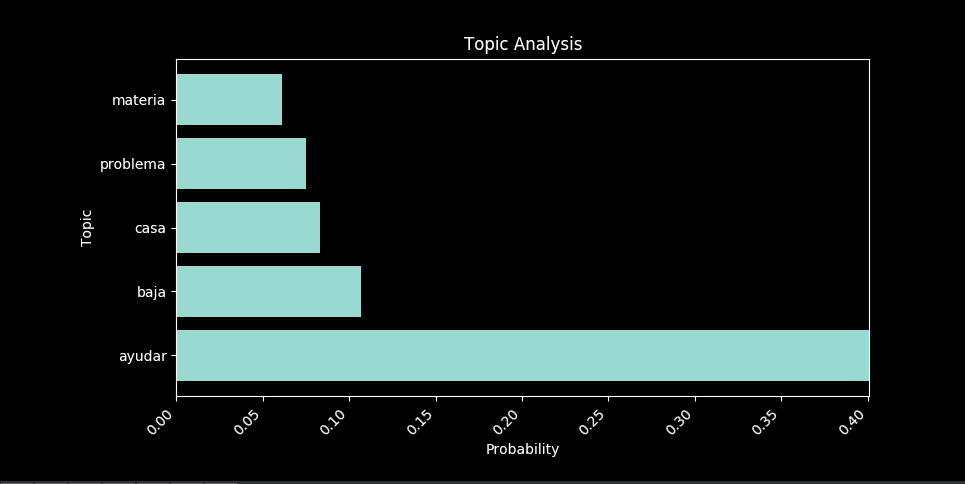
\includegraphics[height=8cm, width=16.5cm]{Latex/Classes/Imagenes/ns_wl-5.png}
            \caption{Resultado \textbf{LDA} con documentos sin \textit{stopwords} y con lemas (e).}
            \label{fig:ns_wl-5}
        \end{figure}
        \begin{figure}[H]
            \centering
            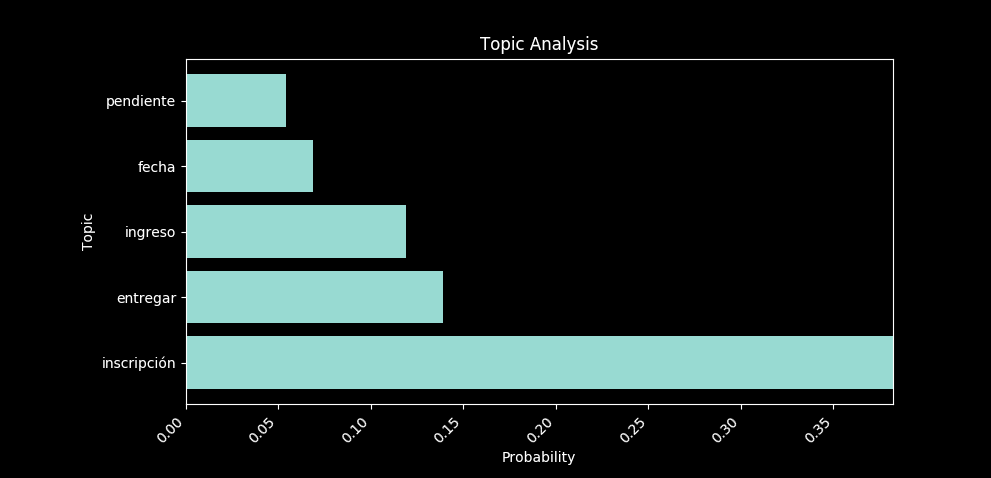
\includegraphics[height=8cm, width=16.5cm]{Latex/Classes/Imagenes/ns_wl-6.png}
            \caption{Resultado \textbf{LDA} con documentos sin \textit{stopwords} y con lemas (f).}
            \label{fig:ns_wl-6}
        \end{figure}
        \begin{figure}[H]
            \centering
            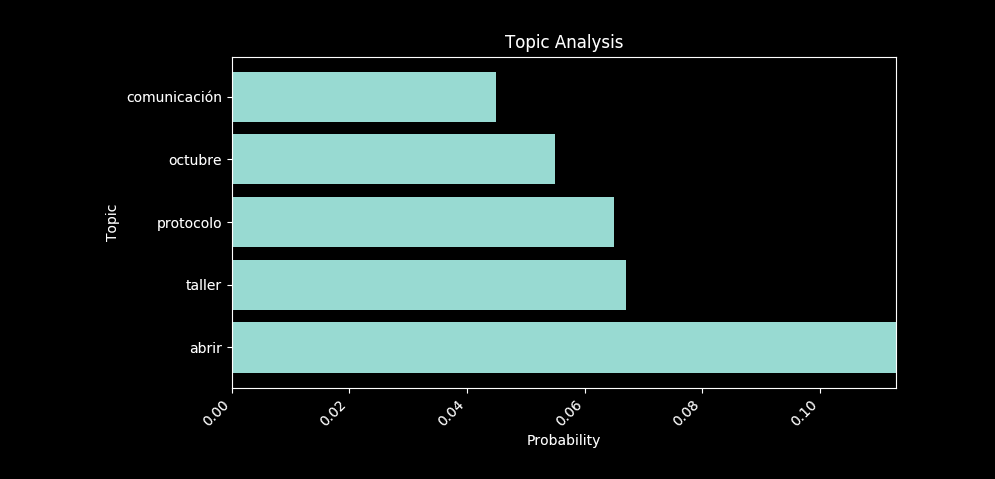
\includegraphics[height=8cm, width=16.5cm]{Latex/Classes/Imagenes/ns_wl-7.png}
            \caption{Resultado \textbf{LDA} con documentos sin \textit{stopwords} y con lemas (g).}
            \label{fig:ns_wl-7}
        \end{figure}
        \begin{figure}[H]
            \centering
            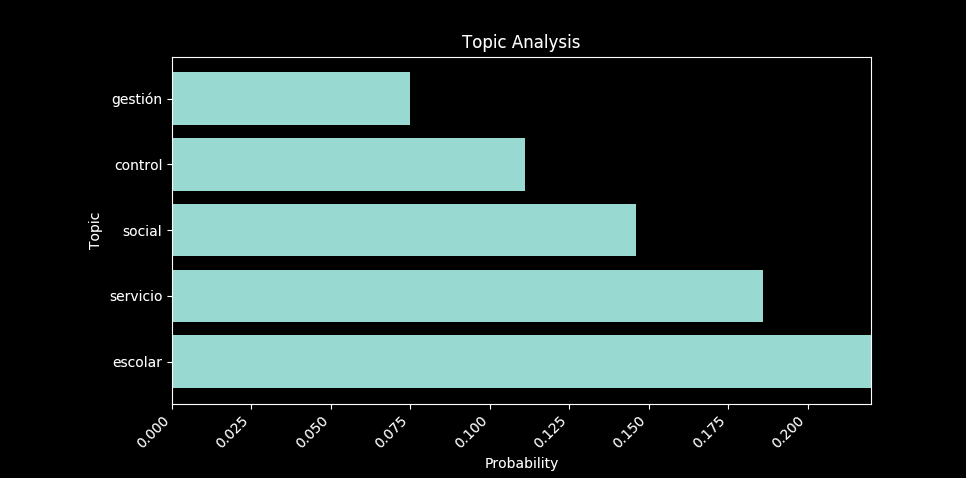
\includegraphics[height=8cm, width=16.5cm]{Latex/Classes/Imagenes/ns_wl-8.png}
            \caption{Resultado \textbf{LDA} con documentos sin \textit{stopwords} y con lemas (h).}
            \label{fig:ns_wl-8}
        \end{figure}
        
    \end{itemize}
\chapter{Anexos}
        
    \section{Anexo I. Análisis de campo}
    
        \subsection{Encuesta}
            Las siguientes preguntas hacen referencia a los procesos para realizar trámites del ámbito de la gestión educativa de la Escuela Superior de Cómputo.
    
            \begin{multicols}{2}
        
                \begin{enumerate}
                    \item ¿Cómo te enteras del procedimiento para llevar a cabo tus trámites?
                    \begin{enumerate}[(a)]
                        \item Compañeros o Amigos
                        \item Página web de la escuela
                        \item Redes sociales
                        \item Semana de inducción
                        \item Atención en ventanilla
                        \item Atención telefónica 
                        \item Otro
                    \end{enumerate}
                
                    \item ¿Has tenido problemas a la hora de realizar algún trámite?
                    \begin{enumerate}[(a)]
                        \item SI
                        \item No
                    \end{enumerate}
                    \item Si la respuesta fue sí, ¿Cuáles consideras que son los 3 principales impedimentos a la hora de realizar un trámite?
                    \begin{enumerate}[(a)]
                        \item Falta de información
                        \item Falta de claridad en el proceso
                        \item Falta de documentación
                        \item Información no actualizada 
                        \item Fuera de tiempo
                        \item Otro
                    \end{enumerate}
                    \item ¿Requeriste más de un medio para poder obtener la información que necesitabas?
                    \begin{enumerate}[(a)]
                        \item SI
                        \item No
                    \end{enumerate}
                    \item ¿Alguna vez has intentado pedir asesoría para realizar un trámite por medio de internet?
                    \begin{enumerate}[(a)]
                        \item SI
                        \item No
                    \end{enumerate}
                    Si la respuesta fue sí, contesta las preguntas 6-9: 
                    \item ¿En qué medio buscaste la asesoría?
                    \begin{enumerate}[(a)]
                        \item Página de facebook
                        \item Messenger de facebook
                        \item Twitter
                        \item Correo electrónico
                        \item Otro
                    \end{enumerate}
                
                    \item ¿En cuanto tiempo te obtuviste la asesoría?
                    \begin{enumerate}[(a)]
                        \item En menos de una hora
                        \item Ese mismo día más tarde
                        \item Días después
                        \item No obtuve una respuesta
                    \end{enumerate}
                
                    \item La información que te proveyeron fue: (Marca las necesarias)
                    \begin{enumerate}[(a)]
                        \item Completa
                        \item Oportuna
                        \item Relevante
                        \item Accesible
                        \item Entendible
                        \item Clara
                        \item Precisa
                        \item Satisfactoria
                    \end{enumerate}
                
                    \item ¿Como fue la experiencia a la hora de solicitar la información?
                    \begin{enumerate}[(a)]
                        \item Muy satisfactoria 
                        \item Buena
                        \item Regular
                        \item Mala
                    \end{enumerate}
                    \item Si las respuestas a través de Facebook Messenger a tus dudas sobre distintos trámites fueran contestadas con prontitud. ¿Qué prioridad de uso le darías a este servicio?
                    \begin{enumerate}[(a)]
                        \item Seria mi primera opción
                        \item Estaría entre mis opciones
                        \item No lo usaría
                    \end{enumerate}
                \end{enumerate}
                
        \end{multicols}
    
        La propuesta de solución a este problema es la creación de un prototipo de agente conversacional popularmente conocido como chatbot proveído a través del aplicativo de facebook para mensajería instantánea “Messenger”, este estará enfocado a la resolución de preguntas frecuentes formuladas por el alumnado de ESCOM.
        
        
        La información recabada en esta encuesta nos será de gran utilidad, por parte de los integrantes y directores del trabajo terminal 2019-A087 le damos las gracias por completar esta encuesta.
    
        \subsection{Resultados}
            \begin{figure}[H]
                \centering
                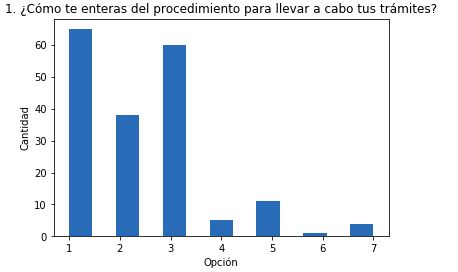
\includegraphics[width=.8\linewidth]{Latex/Classes/Imagenes/1.png}
                \caption{Gráfico de barras: Pregunta 1}
            \end{figure}
            \begin{figure}[H]
                \centering
                \includegraphics[width=.8\linewidth]{Latex/Classes/Imagenes/2.png}
                \caption{Gráfico de barras: Pregunta 2}
            \end{figure}
            \begin{figure}[H]
                \centering
                \includegraphics[width=.8\linewidth]{Latex/Classes/Imagenes/3.png}
                \caption{Gráfico de barras: Pregunta 3}
            \end{figure}
            \begin{figure}[H]
                \centering
                \includegraphics[width=.8\linewidth]{Latex/Classes/Imagenes/4.png}
                \caption{Gráfico de barras: Pregunta 4}
            \end{figure}
            \begin{figure}[H]
                \centering
                \includegraphics[width=.8\linewidth]{Latex/Classes/Imagenes/5.png}
                \caption{Gráfico de barras: Pregunta 5}
            \end{figure}
            \begin{figure}[H]
                \centering
                \includegraphics[width=.8\linewidth]{Latex/Classes/Imagenes/6.png}
                \caption{Gráfico de barras: Pregunta 6}
            \end{figure}
            \begin{figure}[H]
                \centering
                \includegraphics[width=.8\linewidth]{Latex/Classes/Imagenes/7.png}
                \caption{Gráfico de barras: Pregunta 7}
            \end{figure}
            \begin{figure}[H]
                \centering
                \includegraphics[width=.8\linewidth]{Latex/Classes/Imagenes/8.png}
                \caption{Gráfico de barras: Pregunta 8}
            \end{figure}\begin{figure}[H]
                \centering
                \includegraphics[width=.8\linewidth]{Latex/Classes/Imagenes/9.png}
                \caption{Gráfico de barras: Pregunta 9}
            \end{figure}
            \begin{figure}[H]
                \centering
                \includegraphics[width=.8\linewidth]{Latex/Classes/Imagenes/10.png}
                \caption{Gráfico de barras: Pregunta 10}
            \end{figure}
            
            \begin{figure}[H]
                \centering
                \includegraphics[width=.5\linewidth]{Latex/Classes/Imagenes/correlacion.png}
                \caption{Mapa de correlación de variables ente las preguntas de la encuesta}
            \end{figure}
    
    \newpage
    \section{Anexo II. Entrevista }
    \section{Anexo III. Métricas del ajuste de la completitud técnica}
        \begin{enumerate}
            \item Comunicación de Datos
                \begin{description}
                    \item[0:] Aplicación es batch exclusivamente
                    \item[1-2] Impresión o entrada de datos remota
                    \item[3-5] Teleproceso (TP) interactivo
                    \item[3] TP interface a un proceso batch
                    \item[5] La aplicación se interactiva
                \end{description}
            \item Función Distribuída. "Distribuída" significa que los componentes de la aplicación están distribuídos en dos o más procesadores diferentes.
                \begin{description}
                    \item[0:] La aplicación no ayuda a la trasferencia de datos o a la función de procesamiento entre los componentes del sistema
                    \item[1] La aplicación prepara datos para el usuario final de otro procesador
                    \item[2-3] Los datos se preparan para trasferencia, se trasfieren y se procesan en otro componente del sistema
                    \item[4] Igual que 2-3, pero con realimentación al sistema inicial
                    \item[5] Las funciones de procesamiento se realizan dinámicamente en el componente más apropiado del sistema.
                \end{description}
            \item Rendimiento (referido a la importancia de respuesta dentro de todo el sistema)
                \begin{description}
                    \item[0, 3:]Análisis y diseño de las consideraciones del rendimiento son estándar. No se requieren requerimientos especiales por parte del usuario
                    \item[4:]En la fase de diseño se incluyen tareas del análisis del rendimiento para cumplir los requerimientos del usuario
                    \item[5:]Además se utilizan herramientas de análisis del rendimiento en el diseño, desarrollo e instalación
                \end{description}
            \item Configuración utilizada masivamente (referente a la importancia del entorno)
                \begin{description}
                    \item[0, 3:]La aplicación corre en una máquina estándar sin restricciones de operación
                    \item[4:]Restricciones de operación requieren características específicas de la aplicación en el procesador central
                    \item[5:]Además hay restricciones específicas a la aplicación en los componentes distribuídos del sistema.
                \end{description}
            \item Tasas de Transacción (una alta llegada de transacciones provoca problemas más allá de los de la característica 3)
                \begin{description}
                    \item[0, 3:]Las tasas son tales que las consideraciones de análisis de rendimiento son estándares
                    \item[4:]En la fase de diseño se incluyen tareas de análisis de rendimiento para verificar las altas tasas de transacciones
                    \item[5:]Además se utilizan herramientas de análisis del rendimiento.
                \end{description}
            \item Entrada On-Line de datos
                \begin{description}
                    \item[0, 2:]Hasta el 15\% de las transacciones tienen entrada interactiva
                    \item[3, 4:]15\% al 30\% tienen entrada interactiva
                    \item[5:]30\% al 50\% tienen entrada interactiva.
                \end{description}
            \item Diseño para la eficiencia de usuario final
                \begin{description}
                    \item[0:]Sistema batch
                    \item[1, 3:]No se especifican requerimientos especiales
                    \item[4:]Se incluyen tareas de diseño para la consideración de factores humanos
                    \item[5:]Además se utilizan herramientas especiales o de prototipado para promover la eficiencia.
                \end{description}
            \item Actualización On-Line
                \begin{description}
                    \item[0:]Nada
                    \item[1, 2:]Actualización on line de los ficheros de control. El volumen de actualización es bajo y la recuperación fácil.
                    \item[3:]Actualización on line de la mayoría de los ficheros internos lógicos
                    \item[4:]Además es esencial la protección contra la pérdida de datos
                    \item[5:]Además se considera el coste de recuperación de volúmenes elevados.
                \end{description}
            \item Complejidad del procesamiento (esto es complejidad interna más allá de las convenciones de cuenta de entidades de MkII FPA).
                ¿Qué características tiene la aplicación?
                \begin{itemize}
                    \item mucho procesamiento matemático y/o lógico
                    \item muchas excepciones de procesamiento, muchas transacciones incompletas y mucho reprocesamiento de las transacciones
                    \item procesamiento de seguridad y/o control sensitivo
                \end{itemize}
                \begin{description}
                    \item[0:]No se aplica nada de esto
                    \item[1, 3:]Se aplica alguna cosa
                    \item[4:]Se aplican dos cosas
                    \item[5:]Se aplica todo.
                \end{description}
            \item Utilizable en otras aplicaciones (el código se diseña para que sea compartido o utilizable por otras aplicaciones  -no confundir con 13).
                \begin{description}
                    \item[0, 1:]Una aplicación local que responde a las necesidades de una organización usuaria
                    \item[2, 3:]La aplicación utiliza o produce módulos comunes que consideran más necesidades que las del usuario
                    \item[4, 5:]Además, la aplicación se empaquetó y documentó con el propósito de fácil reutilización
                \end{description}
            \item Facilidad de Instalación
                \begin{description}
                   \item[0, 1:]No se requieren por parte del usuario facilidades especiales de conversión e instalación
                   \item[2, 3:]Los requerimientos de conversión e instalación fueron descritos por el usuario y se proporcionaron guías de conversión e instalación
                   \item[4, 5:]Además se proporcionaron y probaron herramientas de conversión e instalación
                \end{description}
            \item Facilidad de Operación
                \begin{description}
                   \item[0:]No se especifican por parte del usuario consideraciones específicas de operación
                   \item[1, 2:]Se requieren, proporcionan y prueban procesos específicos de arranque, backup y recuperación
                   \item[3, 4:]Además la aplicación minimiza la necesidad de actividades manuales, tales como instalación de cintas y papel
                   \item[5:]La aplicación se diseña para operación sin atención
                \end{description}
            \item Puestos Múltiples. Añadir puntos por cada uno de los siguientes factores
                \begin{description}
                   \item[0:]El usuario no requiere la consideración de más de un puesto
                   \item[1:]De uno a cuatro puestos
                   \item[2:]Cinco o más puestos
                   \item[1:]Se proporciona documentación y plan de apoyo para soportar la aplicación en varios lugares
                   \item[2:]Los puestos están en países diferentes
                \end{description}
            \item Facilidad de Cambio (esfuerzo específico de diseño para facilitar cambios futuros). Añadir puntos por cada uno de los siguientes factores
                \begin{description}
                   \item[0:]No hay requerimientos especiales del usuario para minimizar o facilitar el cambio
                   \item[1, 3:]Se proporciona capacidad de consulta flexible
                   \item[4, 5:]Datos importantes de control se mantienen en tablas que son actualizadas por el usuario a través de procesos on-line interactivos.
                \end{description}
            \item Requerimientos de otras Aplicaciones
                \begin{description}
                   \item[0:]El sistema es stand-alone
                   \item[1, 4:]Requerimientos del sistema para interfaces o compartición de datos deben ser sincronizados con otras aplicaciones
                   \item[5:]Se deben sincronizar los requerimientos del sistema con cuatro o más aplicaciones
                \end{description}
            \item Seguridad, Privacidad y Auditoría. Añadir puntos por cada uno de los siguientes factores
                \begin{description}
                   \item[1:]Si el sistema debe cumplir requerimientos personales (incluso legales) de privacidad
                   \item[1:]Si el sistema debe cumplir requerimientos especiales de auditoría
                   \item[1, 2:]Si el sistema debe cumplir requerimientos excepcionales de seguridad para prevenir pérdidas de naturaleza financiera o militar
                   \item[1:]Si se requiere el criptográfico de los datos de las comunicaciones
                 \end{description}
            \item Necesidad de Adiestramiento al Usuario
                \begin{description}
                   \item[0:]Si no es necesario material ni cursos
                   \item[1, 4:]Si se requiere entrenamiento especial o se proporcionan facilidades de ayuda on-line
                   \item[5:]Se requiere un sistema separado de entrenamiento o simulador
                \end{description}
    
            \item Uso directo de otras empresas
                \begin{description}
                   \item[0:]No existe otra empresa conectada al sistema
                   \item[1:]Los datos se envían o reciben de empresas conocidas
                   \item[2:]Empresas conocidas están conectadas al sistema en modo de lectura solamente
                   \item[3, 4:]Empresas conocidas están conectadas directamente al sistema con capacidad de actualización on-line
                   \item[5:]Empresas desconocidas (público en general o un grupo demasiado extenso como para ser adiestrado) pueden acceder al sistema
                \end{description}
            \item Documentación. Contar 1 por cada tipo de documento listado a continuación que se entrega al final del proyecto.
                \begin{itemize}
                    \item Especificación Funcional del Sistema (datos y procesos)
                    \item Especificación Técnica del Sistema
                    \item Documentación del programa (al menos diagramas de flujo)
                    \item Librería de Elementos de Datos
                    \item Elemento de Datos/ Registro/ X-referencia del programa
                    \item Manual de usuario
                    \item Folleto de información general del sistema
                    \item Librería de datos de prueba
                    \item Material de curso de adiestramiento al usuario
                    \item Documentos de coste/beneficio del sistema
                    \item Informe de petición de cambios y errores
                \end{itemize}
                Se calcula el grado de influencia utilizando la siguiente tabla
                \begin{enumerate}
                   \item si 0-2 tipos de documento
                   \item si 3-4
                   \item si 5-6
                   \item si 7-8
                   \item si 9-10
                   \item si 11-12 tipos de documento
                \end{enumerate}
        \end{enumerate}
    
    


%%%%%%%%%%%%
% APPENDIX %
%%%%%%%%%%%%
\appendix

%%%%%%%%%%%%%%
% REFERENCES %
%%%%%%%%%%%%%%
%\bibliographystyle{apalike}
%\bibliography{Bibliografia/referencias}

\end{document}

